\documentclass[a4paper, 11pt, normalem]{report}

\usepackage{../../../LaTeX-Templates/Notes}

\newcommand\answerbox{%%
    \fbox{\rule{0.8in}{0pt}\rule[-0.5ex]{0pt}{3ex}}}

\newcommand\halfbox{%%
    \fbox{\rule{0.36in}{0pt}\rule[-0.25ex]{0pt}{3ex}}}

\title{Foundations of Physics 2B \\ Thermodynamics \vspace{-20pt}}
\author{Dr Peter Swift}
\date{\vspace{-15pt}Michaelmas Term 2017}
\rhead{\hyperlink{page.1}{Go to TOC}}

\begin{document}

\maketitle
\thispagestyle{fancy}

\tableofcontents

\chapter{}
\section{Intro}
This course will frame concepts in concrete maths from last year

Laws:
\begin{itemize}
  \item Zeroth establishes the meaning of temperature
  \item First is a statement of energy conservation [we can only break even]
  \item Second defines entropy -- why things do or do not happen
  \begin{itemize}
    \item[--] Entropy measures energy quality [you can only break even at 0 K]
  \end{itemize}
  \item Third doesn't define thermodynamic property; tells us we can't get to 0 K
\end{itemize}

Thermodynamics developed by engineers wanting to develop machines that turn heat to work \\
Wanted most work for least effort \\
Subject developed had a number of under-ranging consequences \\
When it emerged, atoms were unknown -- considered average properties of bulk material \\
There was no attention paid to what was inside \\
Macroscopic approach to look at 'black box':
\begin{itemize}
  \item[--] This approach is general and difficult to 'see the point' \\
  All good having relationships about heat capacities and expansicities but tells us nothing about the physics
  \item[e.g.] why a material has a certain temperature dependence for its heat capacity
\end{itemize}

Opening the black box gets microscopic picture (atomic) but this can be very detailed ($N_A \approx 6 \times 10^23$) \\
Statistical mechanics instead looks at average properties of all atoms in the thermodynamic limit

\subsection{Counting Molecules -- simpler than recording position and motion  as fewer DoFs}
Lecture theatre has $10^29$ molecules ($3 \times 10^6$ litres of air) \\
A 10GhZ processor can count $10^17$ molecules per year (each cycle counts one) $\approx 3 \times 10^11$ years to count all molecules \\
Thermodynamic limit -- things tend to the average (to infinity)

\subsection{Rains drops hit small and large roof:}
Fluctuations in force smooth out, even through force increasing \\
Consider pressure, $p = \frac{F}{A}$, same in both cases if you consider the average \\
Thermodynamic limit -- $A \to \infty$

\section{Thermo Systems and States}
\begin{tabular}{c|c|c}
     & Extensive -- System Extent & Intensive -- Independent \\
     \hline
     \multirow{2}{7em}{\answerbox} & Volume, V & Temp, T \\
     & Energy, U & Pressure, P \\
     \hline
     \multirow{2}{7em}{\halfbox \halfbox} & $V = V_A = V_B = \frac{V}{2}$ & $T^* = T_A = T_B = T$ \\
     & $U = U_A = U_B = \frac{U}{2}$ & $p^* = p_A = p_B = p$
\end{tabular}

Relate properties by equation of state, $f(p,V,T) = 0$ \\
Most well known as the ideal gas law: $pV = nRT$

\section{Thermal Equilibrium (TE), Heat, and Temperature}
Can prepare sample of gas by suitable treatment to take a range of values of pressure and volume
\begin{equation*}
    p_{1}V_{1} = a > b = p_{2}V_{2} \text{ -- Sample 1 is hotter than Sample 2}
\end{equation*}
Equation of state, $pV = f(T)$

Heat is thermal energy in transit, heat transferred from hot to cold (under its own action) \\
In transit is important -- can't say object contains an amount of heat \\
Addition/subtraction of heat changes temperature \\
If two objects have the same temperature, they're in TE

Heat capacity -- $\Delta Q = mc\Delta T$ \\
More rigorously, a small change, dT, in a substance's temperature, requires the addition/subtraction of a differention and of heat,  $\delta Q$:
\begin{equation*}
    \delta Q = mcdT
\end{equation*}
Capital C: Heat capacity of whole substance \\
Lower c: Specific heat capacity per unit mass/mole \\
$C = mc$

Total heat energy to change temperature, $T_1 \to T_2$:
\begin{equation*}
    \Delta Q = \int_{T_{1}}^{T_{2}} \delta Q = \int_{T_1}^{T_2} mcdT
\end{equation*}
Most changes take place whilst some other property is held constant:
\begin{gather*}
    C_{V} = \Big(\frac{\p Q}{\p T}\Big)_{V};~~ C_{p} = \Big(\frac{\p Q}{\p T}\Big)_{p}
    C_{p} > C_{V}
\end{gather*}
Work is needed to keep at constant pressure -- work is a form of energy so requires more heat energy in to get to the same temperature at constant pressure

\chapter{}
\section{Zeroth Law}
\emph{"If two system are separately in TE with a third system, they must be in TE with each other"}

If heat flows between two systems, they can't spontaneously turn back to initial states. \\
If two objects are at the same temperature, they're in TE \\
This defines the arrow of time

Thermometers have a low heat capacity relative to the object they're measuring

\section{Relevant Maths}
Thermodynamics is concerned with properties that change \\\
Changing one (e.g. temp) will affect others (e.g. pressure) but might hold some more (e.g. volume) constant \\
Always denote what is held constant explicitly
\begin{equation*}
    C_p = \Big(\frac{\p Q}{\p T}\Big)_p \neq \Big(\frac{\p Q}{\p T}\Big)_V = C_V
\end{equation*}

\subsection{}
Kinetic energy in gases: $U = \frac{1}{2}m<v>^2 = \frac{3}{2}Nk_{b}T$ \\
Look at ideal gases for simplification:
\begin{gather*}
    pV = nRT;~~ n = \frac{N}{N_{A}};~~ R = N_{A}k_{b} \\
    U = \frac{3}{2}Nk_{b}T = \frac{3}{2}pV \\
    \Big(\frac{\p U}{\p V}\Big)_T = 0;~~ \Big(\frac{\p U}{\p V}\Big)_p = \frac{3}{2}p
\end{gather*}
Look at First Law:
\begin{gather*}
    dU = T\,ds - p\,dV \\
    \Big(\frac{\p U}{\p V}\Big)_S = -p
\end{gather*}
Now consider the total differential of $z = f(x,\,y)$, $z = Z(x,\,y)$, or $f(x,\,y,\,z) = 0$ \\
This has two independent variables
\begin{equation*}
    dz = \Big(\frac{\p z}{\p x}\Big)_y dx + \Big(\frac{\p z}{\p y}\Big)_x dy
\end{equation*}
\newpage
\begin{wrapfigure}{r}{0.35\textwidth}
    \begin{center}
        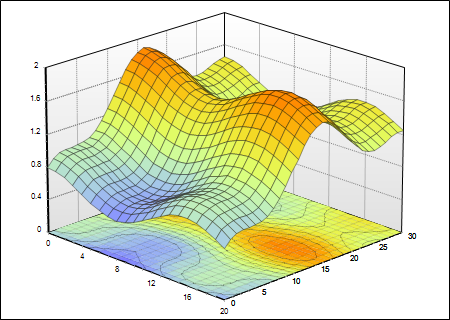
\includegraphics[scale=0.35]{Surface.png}
    \end{center}
\end{wrapfigure}
Infinitesimal change in z resulting from infinitesimal changes in x and y \\
Z represents a surface

Consider an intersection of the surface in the x-z plane at some y

Rather than consider the value of z, we look at the shape at any point of the lines of intersection with planes constant x or y

\subsection{}
For $p = p(V,\,T)$:
\begin{gather*}
    dp = \Big(\frac{\p p}{\p V}\Big)_T dV + \Big(\frac{\p p}{\p T}\Big)_V dT \\
    pV = nRT ~~\implies \\
    \Big(\frac{\p p}{\p V}\Big)_T = -\frac{RT}{V^2};~~ \Big(\frac{\p p}{\p T}\Big)_V = \frac{R}{V} \\
    dp = -\frac{RT}{V^2}dV + \frac{R}{V}dT \\
    dp = \frac{RT}{V}\Big(- \frac{dV}{V} + \frac{dT}{T}\Big)~~ \Big[p = \frac{RT}{V}\Big] \\
    \frac{dp}{p} = - \frac{dV}{V} + \frac{dT}{T} \\
    d(\ln{p}) = -d(\ln{V}) + d(\ln{T})~~ \Big[\frac{d(\ln{x})}{dx} = \frac{1}{x} \Big]
\end{gather*}

\textbf{Proof 2.2.2.1:}\\
x, y, and z related via $f(x,\,y,\,z)$
\begin{gather*}
    x = X(y,\,z)~;~ y = Y(x,\,z) \\
    dx = \Big(\frac{\p X}{\p y} \Big)_z dy + \Big(\frac{\p X}{\p z} \Big)_y ~;~ dy = \Big(\frac{\p Y}{\p x} \Big)_z dx + \Big(\frac{\p Y}{\p z} \Big)_x dz \\
    dx = \Big(\frac{\p x}{\p y} \Big)_z \Big(\frac{\p y}{\p x} \Big)_z dx + \Bigg[\Big(\frac{\p x}{\p y} \Big)_z \Big(\frac{\p y}{\p z} \Big)_x + \Big(\frac{\p x}{\p z} \Big)_y \Bigg] dz \\
    dx = M(x,\,y)\,dx + N(x,\,y)\,dz
\end{gather*}
For $M = 1$:
\begin{equation*}
    \Big(\frac{\p x}{\p y} \Big)_z \Big(\frac{\p y}{\p x} \Big)_z = 1 \text{ -- Reciprocal Theorem}
\end{equation*}
For $N = 0$:
\begin{gather*}
    \Big(\frac{\p x}{\p y} \Big)_z \Big(\frac{\p y}{\p z} \Big)_x + \Big(\frac{\p x}{\p z} \Big)_y = 0 ~~ \Bigg[ \times \Big(\frac{\p z}{\p y} \Big)_y \Bigg] \\
    \Big(\frac{\p x}{\p y} \Big)_z \Big(\frac{\p y}{\p z} \Big)_x \Big(\frac{\p z}{\p y} \Big)_y + 1 = 0 \\
    \Big(\frac{\p x}{\p y} \Big)_z \Big(\frac{\p y}{\p z} \Big)_x \Big(\frac{\p z}{\p y} \Big)_y = -1 \text{ -- Reciprocity Theorem (Cyclic)}
\end{gather*}
Well-behaved functions (as above) are exact differentials

For $z = f(x,\,y)$ with two independent variables
\begin{equation*}
    dz = M(x,\,y)\,dx + N(x,\,y)\,dy
\end{equation*}
If exact:
\begin{gather*}
    \Big(\frac{\p M}{\p y} \Big)_x = \Big(\frac{\p N}{\p x} \Big)_y \\
    \frac{\p}{\p y}\Bigg[\Big(\frac{\p M}{\p y} \Big)_x \Bigg]_y = \frac{\p^2 z}{\p x \p y} \equiv \frac{\p}{\p x}\Bigg[\Big(\frac{\p N}{\p x}\Big)_y \Bigg]_x = \frac{\p^2 z}{\p x \p y}
\end{gather*}
For exact functions, the order of the second derivatives doesn't matter. \\
These are \emph{line integrals}.
\begin{equation*}
    I = \int_{1}^{2} dz = \int M(x,\,y)\,dx + \int N(x,\,y)\,dy = Z_2 - Z_1
\end{equation*}
Parts can be integrated independently and the answer doesn't depend on the path \\
These correspond to functions of state in thermodynamics (p, V, T)

If $\frac{\p^2 z}{\p x \p y} \neq \frac{\p^2 z}{\p y \p x}$, this is inexact, and a \emph{point function}. \\
The value of the integral depends on the path (W, Q)

dV - incremental volume change \\
Total volume change from state 1 to 2:
\begin{equation*}
    \int_{1}^{2} dV = V_2 - V_1 = \Delta V
\end{equation*}
If we return to original state, the path is closed:
\begin{equation*}
    \oint dV = 0
\end{equation*}
The work between two states is path dependent:
\begin{equation*}
    W_{1 \to 2} = \int_{1}^{2} \delta W \neq W_2 - W_1
\end{equation*}
\begin{wrapfigure}{l}{0.4\textwidth}
    \begin{center}
        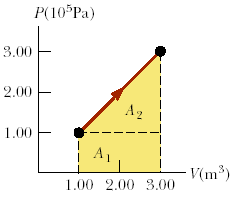
\includegraphics[scale=0.6]{WorkPV.png}
    \end{center}
    \vspace{-120pt}
\end{wrapfigure}

Differential works along the path are added.
\begin{gather*}
\left.\begin{aligned}
       \Delta V_1 &= V_2 - V_1 \\
       \Delta V_2 &= V_2 - V_1
      \end{aligned}
\right\}
    \quad \text{exact dV, path independent} \\
    W_1 \neq W_2 ~ \text{ -- areas are different, so inexact } \delta W
\end{gather*}

\newpage
\subsection{}
\begin{wrapfigure}{r}{0.4\textwidth}
    \begin{center}
        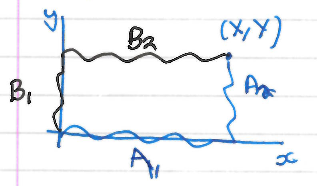
\includegraphics[scale=0.5]{XYCord.png}
    \end{center}
\end{wrapfigure}
Consider $\delta F = x\,dx + x\,dy$ (inexact) with two paths for $(0,\,0) \to (X,\,Y)$

Path A: $(0,\,0) \to (X,\,0) \to (X,\,Y)$ \\
Path B: $(0,\,0) \to (0,\,Y) \to (X,\,Y)$
\begin{flalign*}
    A &=
    \begin{cases}
        A_1 & \int_{A_1} \delta F = \int_{0}^{X} x\,dx + \cancel{\int_{0}^{0} x\,dy}^{dy = 0} = \frac{X^2}{2} \\
        +   & \\
        A_2 & \int_{A_2} \delta F = \cancel{\int_{X}^{X} X\,dx}^{dx = 0} + \int_{0}^{Y} X\,dy = [Xy]_{0}^{Y} = XY
    \end{cases}
    \\\\
    \int_{A} &\delta F = \int_{A_1} + \int_{A_2} = \frac{X^2}{2} + XY ~~;~~ \int_{B} \delta F = \frac{X^2}{2}
\end{flalign*}

\chapter{}
\section{Work and Internal Energy}
Work done depends on path (inexact) and comes when motion opposes a force (push a box against friction)

Work done on a system - compression of a gas - is positive \\
Work done by a system - expansion of a gas - is negative
\begin{equation*}
    \delta W = -p\,dV = -p_{0}(V_f - V_i)
\end{equation*}
In compression:
\begin{equation*}
    V_f < V_i ~;~ \delta W = -p( < 0) = +\text{ve}
\end{equation*}
\emph{Internal energy is the sum of all the internal Degrees of Freedom (total energy of thermodynamic state)}

Joule discovered mechanical equivalent of heat: dropped a weight that turned a paddle in water and measured the temperature change.

Furthermore, we have two objects not in TE, can connect a heat engine to get work out. \\
Therefore heat, work, and internal energy are related by the First Law.

\section{The First Law}
 \emph{Energy is a measure of a system's capacity to do work}

The types of work:
\begin{itemize}
    \item Configuration - a system's configuration is changed by altering thermodynamic conditions ($\delta W = -p\,dV ~;~ \delta W = \gamma\,dA = m\,dB$)
    \item Dissipative - gets turned into internal energy (if non-zero, gets lost as a form of converting heat to work)
    \item Adiabatic - done on a system in thermal isolation
\end{itemize}

The first law is a statement of conservation of energy - do work and add heat to a substance, and its internal energy changes:
\begin{gather*}
    \Delta U = \Delta Q + \Delta W \\
    dU = \delta Q + \delta W
\end{gather*}
A system is in a macrostate described by two of p,V, and T related by an equation of state. \\
We must assert that any given state has the same total energy, U. [internal energy is the sum of all the DoFs]

First Law:
\begin{itemize}
    \item \emph{If a system moves from initial state, i, to final state, f, via adiabatic paths, the work done is the same for all paths}
\end{itemize}
Independence of work $\implies$ internal energy is a function of state
\begin{equation*}
    \int_{i}^{f} dU = U_f - U_i = W_{if}^{ad}
\end{equation*}
Do work on a system (compress): $W_{if}^{ad} > 0 ~;~ U_f > U_i$

Experiments show when a system changes from state i to state f by different adiabatic paths, as measured by the change in the level of a weight, the work done is the same

We empirically find that the system is not thermally isolated, the work done is not the same as the internal change.
\begin{equation*}
    W_{if} \neq U_f - U_i ~;~ U_f - U_i = Q_{if} + W_{if}
\end{equation*}
Add or remove heat as it is not isolated and do work \\
Q and W depend on the path so:
\begin{equation*}
    dU = \delta Q + \delta W = \delta Q - p\,dV
\end{equation*}

\section{Heat Capacity Relationships}
\begin{equation*}
    \delta Q = C\,dT ~;~ C_{V} \Big(\frac{\p Q}{\p T}\Big)_{V} ~;~ C_{p} = \Big(\frac{\p Q}{\p T} \Big)_{p}
\end{equation*}

\textbf{Proof:}\\
How does heat capacity change internal energy of a gas?

Internal energy is our fourth function of state (U only depends on the state the system is in, not how it got there) \\
As we know, an equation of state can be used to express one thermodynamic coordinate in terms of others:
\begin{equation*}
    U = U(V,\,T) ~;~ p = p(V,\,T)
\end{equation*}
Total differential:
\begin{gather*}
    dU = \Big(\frac{\p U}{\p T} \Big)_V dT + \Big(\frac{\p U}{\p V} \Big)_T dV \\
    dU = \delta Q - p\,dV \\
    \delta Q = \Big(\frac{\p U}{\p T} \Big)_V dT + \Bigg[\Big(\frac{\p U}{\p V} \Big)_T + p \Bigg]\,dV
\end{gather*}
Divide by dT when the volume is constant (V = 0) and take $\lim_{dT \to 0}$:
\begin{gather*}
    \frac{\delta Q}{dT} = \Big(\frac{\p U}{\p T} \Big)_{V} \frac{dT}{dT} + \Bigg[\Big(\frac{\p U}{\p V} \Big)_T + p \Bigg]\frac{0}{dT} \\
    \Big(\frac{\p Q}{\p T} \Big)_V = \Big(\frac{\p U}{\p T} \Big)_{V} \\
    \iff V = c \implies C_{V} = \Big(\frac{\p Q}{\p T} \Big)_{V} = \Big(\frac{\p U}{\p T} \Big)_{V}
\end{gather*}
Divide by dT at constant p and take $\lim_{dT \to 0}$:
\begin{gather*}
    \frac{\delta Q}{dT} = \Big(\frac{\p U}{\p T} \Big)_{V} \frac{dT}{dT} + \Bigg[\Big(\frac{\p U}{\p V} \Big)_T + p \Bigg]\frac{dV}{dT} \\
    \Big(\frac{\p Q}{\p T} \Big)_{p} = \Big(\frac{\p U}{\p T} \Big)_{V} + \Bigg[\Big(\frac{\p U}{\p V} \Big)_T + p \Bigg] \Big(\frac{dV}{dT} \Big)_{p} \\
    C_p = C_V + \Bigg[\Big(\frac{\p U}{\p V} \Big)_T + p \Bigg] \Big(\frac{dV}{dT} \Big)_{p}
\end{gather*}

\subsection{Find a relation for Cp and CV for an ideal gas}
\begin{gather*}
    pV = RT ~;~ \Big(\frac{\p U}{\p T} \Big)_{p} = \frac{R}{p} ~;~ U = U(T) \\
    \Big(\frac{\p U}{\p V} \Big)_{T} = 0 \implies C_p = C_V + [0 + p]\frac{R}{p} \\
    \therefore C_p = C_V + R
\end{gather*}

\section{Quasi-State and Reversibility}
All physical laws are reversible \\
e.g. molecules bouncing off a container forwards or backwards

In the real world, certain outcomes are much more likely - can always find ways to convert energy to heat than anything else. \\
This heat is hotter than surroundings so disspiates and tends to TE

Thermodynamics reversibility is when we can change the direction by making some infinitesimal change to a system property

Things are reversible if they quasi-static - happen really slowly

\chapter{}
Processes are quasi-static (no shock waves) - very slow and also have finite temperature differences
\begin{itemize}
    \item[] isobaric - constant pressure
    \item[] isothermal - constant temperature
    \item[] isochoric - constant volume
    \item[] adiabatic - thermally isolated
\end{itemize}
Isobaric heating, supply energy to raise at constant pressure:
\begin{equation*}
    C_p = \Big(\frac{\delta Q}{\delta T}\Big)_p ~;~ \Delta Q = \int C_p \, dT
\end{equation*}

Which way does heat flow during a reversible isothermal expansion of an ideal gas?

Naively add heat ($\Delta Q > 0$) to expand the gas \\
Use the first law: $dU = \delta Q + \delta w = \delta Q - p\,dV$

$V_1 \to V_2 > V_1$ in expansion \\
Isothermal so $dT = 0$ (ideal gas, $U = U(T)$) $\therefore dU = 0$
\begin{gather*}
    dU = U_2 - U_1 = U_{2}(T_{0}) - U_{1}(T_{0}) = 0 \\
    \delta Q = p\,dV \implies Q_{1\to2} = \int_{V_{1}}^{V_{2}} p\,dV \\
    pV = RT_0 \\
    Q_{1\to2} = \int_{V_{1}}^{V_{2}} \frac{RT_{0}\,dV}{V} = RT_{0}\Big[\ln V \Big]_{V_{1}}^{V_{2}} = RT_{0}\ln\bigg[\frac{V_{2}}{V_1}\bigg]
\end{gather*}
As $V_2 > V_1 ~;~ \frac{V_2}{V_1} > 1 ~;~ \ln(> 1) > 0$ \\
i.e. heat input is inline with expectations

\section{Proof of Equation of State for Adiabatic Process}
For ideal gases:
\begin{gather*}
    pV^{\gamma} = K \\
    dU = \delta Q - p\,dV
\end{gather*}
But remember, $dU = C_V \, dT$
\begin{gather*}
    \delta Q = C_V \, dT + p\,dV \\
    C_p - C_V = R \\
    dT = \Big(\frac{\delta T}{\delta V} \Big)_p dV + \Big(\frac{\delta T}{\delta p} \Big)_V dp \\
    pV = RT \implies dT = \frac{p}{R}dV + \frac{V}{R}dp \\
    \delta Q = C_p dT - R\,dT + p\,dV \\
    \delta Q = C_p dT - \cancel{p\,dV} - V\,dp + \cancel{p\,dV} \\
    \delta Q = C_p dT - V\,dp
\end{gather*}
For adiabatic processes, $\delta Q = 0$:
\begin{gather*}
    dT = -\frac{p}{C_V}dV ~;~ dT = \frac{V}{C_p}dp \\
    -\frac{p}{C_p}dV = \frac{V}{C_V}dp \\
    \int \frac{dp}{p} = -\frac{C_p}{C_V}\int \frac{dV}{V} \\
    \gamma = \frac{C_p}{C_V} \implies \\
    \ln p = -\gamma \ln V + C \\
    p = V^{-\gamma}K \\
    pV^{\gamma} = K
\end{gather*}

\section{Heat Engines}
We know turning work to heat is easy but the reverse is more difficult \\
(rotate a paddle in a fluid, it will warm the fluid; but heating the fluid won't rotate the paddle)

Use a heat engine to produce work from temperature difference between reservoirs \\
Heat is taken in at high temperature, some heat is converted to work, and remaining heat is rejected at low temperature (not always obvious - could be to the environment)

Circular path in pV diagram: Path in some thermodynamic states undergoes work interactions, changing thermodynamic conditions (p, V, T) as it state moves round path, and it reutns to its initial states

Steam power plant is best desciption of 'work device'

\section{The Second Law}
This is quite important for all of science - underpins whole understanding of why change happens

Encapsulates understanding of heat engines (heat from work is easy) \\
The Second Law places direction on a process and likelihood it will happen \\
(Energy conservation doesn't mean a process won't happen, it is just unlikely)
\begin{gather*}
    \underbrace{\oint \delta W > 0 \implies \Delta Q < 0}_{\text{Work produces heat}} \\
    \underbrace{\oint \delta W < 0 \implies \Delta Q > 0}_{\text{Heat produces work}}
\end{gather*}
Introduce entropy later on to explain inadequecy of first law \\
Tells us energy quality: the higher the energy quality, the more potential is has.

\section{Clausius Statement}
\emph{It is impossible to devise a process whose sole result is the transfer of heat from cold to hot}

(Nature is asymmetric - heat only goes hot to cold spontaneously, i.e. it will occur by itself)

\section{Kelvin-Planck Statement}
\emph{It is impossible to construct a device that operates in a cycle producing positive work, that only operates with on heat reservoir}

(Tax exists on conversion of heat to work - always some residual heat to expel to cold)

\underline{These two statements are logically similar}

\begin{wrapfigure}{l}{0.4\textwidth}
    \begin{center}
        \vspace{-10pt}
        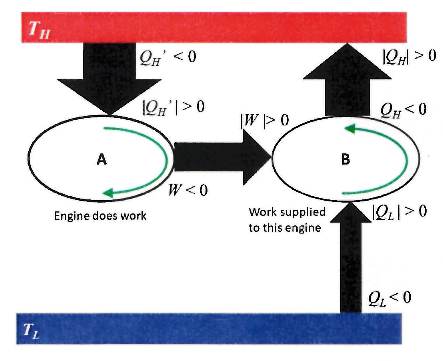
\includegraphics[scale=0.4]{KelvinClause.png}
        \vspace{-70pt}
    \end{center}
\end{wrapfigure}

Two engines have some hot source, $T_H$, but A has no sink \\
The work produced by A drives a fridge, which takes heat from cold to hot

This returns more energy to hot than originally taken \\
Overall, heat is taken from cold to hot, violating the Clausius Statement
\begin{gather*}
    dU = 0 \\
    \delta Q = - \delta W \implies -W_A = |Q_{H}'| ~~ (1) \\
    |W| + |Q_{L}| = -Q_{H} ~~ (2) \\
    (1) + (2) \implies |W| + |Q_{L}| = |Q_{H}| \implies |Q_{H}'| + |Q_{L}| = |Q_{H}| \\
    |Q_{H}'| < |Q_{H}|
\end{gather*}
There is more heat returned to hot, violating Clausius

\begin{wrapfigure}{r}{0.4\textwidth}
    \begin{center}
        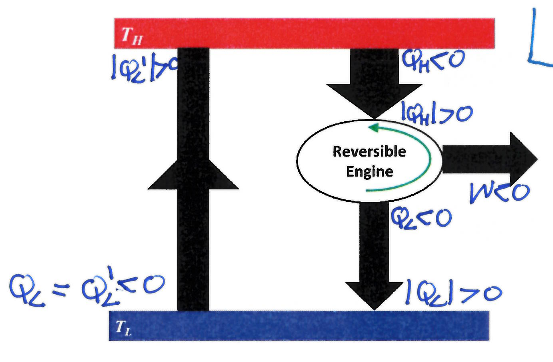
\includegraphics[scale=0.35]{ClausKelvin.png}
    \end{center}
\end{wrapfigure}

We assume all heat dumped in the cold reservoir by the engine spontaneously gets returned to the hot reservoir, violating Clausius \\
The net effect is that the engine only interacts with the hot reservoir, violating Kelvin-Planck

i.e. all heat is converted to work
\begin{gather*}
    dU = 0 \to \delta Q = - \delta W \\
    |Q_{H}| + W + Q_{L} = \\
    -W = |Q_{H}| - |Q_{L}|
\end{gather*}
$|Q_{L}'|$ to hot so $Q_{H} + |Q_{L}'| = Q_{H} + |Q_{L}|$ is only heat removed\\
This is the same as the work done

\chapter{}
\section{Efficiencies}
How much energy in the form of work is got out of a device for a given amount of heat input?

\begin{wrapfigure}{r}{0.4\textwidth}
    \begin{center}
        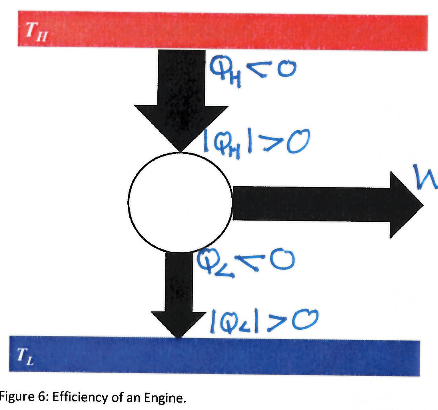
\includegraphics[scale=0.4]{Efficient.png} \\
        \vspace{50pt}
        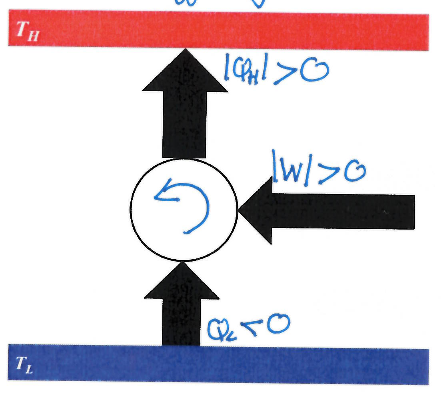
\includegraphics[scale=0.4]{CoP.png}
        \vspace{-160pt}
    \end{center}
\end{wrapfigure}
The first law is a cycle
\begin{gather*}
    dU = \delta Q + \delta W \\
    \int \delta W = - \int \delta Q \\
    \Delta W = - (|Q_H| + Q_L) = -(|Q_H| - |Q_L|) \\
    \eta = \frac{|W|}{Q_H} = \frac{|Q_H| - |Q_L|}{|Q_H|} \\
    \eta = 1 - \frac{|Q_L|}{|Q_H|} \\
    \text{Efficiency } = \eta = \frac{\text{Product}}{\text{Expense}} \\
    \eta = \frac{|\text{Work}|}{\text{Heat Input}} \\
    \eta = \frac{|Q_H| - |Q_L|}{|Q_{H}|} = 1 - \frac{|Q_L|}{|Q_H|}
\end{gather*}
Second law told us $|Q_L| > 0$ always must have a cold sink
$$\eta \neq 1$$
This allows us to define a thermodynamic temperature \\
Relate reservoir heat ineractions to the temperature, T, in Kelvin

Fridge takes heat cold to hot:
\begin{equation*}
    CoP_{L} = \frac{Q_L}{W}
\end{equation*}
Supply work to remove heat from cold \\
Heat pump:
\begin{equation*}
    CoP_H = \frac{|Q_H|}{W}
\end{equation*}
Heat pumps are the most efficient form of heating

\begin{wrapfigure}{l}{0.4\textwidth}
    \begin{center}
        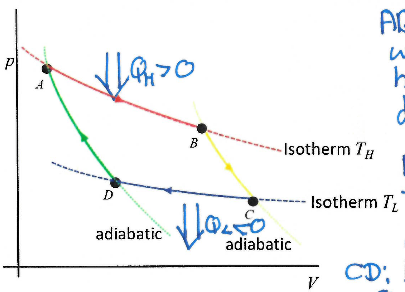
\includegraphics[scale=0.4]{Adiab.png}
        \vspace{-20pt}
    \end{center}
\end{wrapfigure}

AB: Isothermal expansion when working fluid is in contact with the hot reservoir
\begin{equation*}
    T_A = T_B = T_H ~;~ dU = 0 ~;~ Q_H = Q_{AB} > 0 ~;~ W_{AB} < 0
\end{equation*}

BC: Adiabatic expansion from $T_H$ to $T_L$ \\
          $W_BC < 0$ and internal energy also decreases [$dU = \delta Q + \delta W$]

CD: Isothermal compression at $T_L$ \\
          $Q_L < 0 ~~;~~ |W_{CD}| > 0$

DA: Adiabatic Compression \\
          $|W_{DA}| > 0 ~~;~~ dU > 0$

Consider AB: $dU = 0$ (constant temperature of ideal gas) $\therefore dU = \delta Q + \delta W$
\begin{gather*}
    Q_H = = -W_{AB} = - \int_{V_{A}}^{V_B} (-p\,dV) = \int_{V_A}^{V_B} \frac{RT_{H}}{V}dV \\
    Q_H = RT_{H}\ln\Big(\frac{V_B}{V_A}\Big) > 0
\end{gather*}

Now consider CD:
\begin{gather*}
    Q_L = -W_{CD} = - \int_{V_C}^{V_D} (-p\,dV) \\
    Q_L = -RT_L \ln\Big(\frac{V_C}{V_D}\Big) < 0 \\
    \frac{Q_H}{|Q_L|} = \frac{RT_{H}\ln\big(\tfrac{V_B}{V_A}\big)}{\big|-RT_L \ln\big(\tfrac{V_C}{V_D}\big)\big|} = \frac{T_H}{T_L} \cancel{\frac{\ln\big(\tfrac{V_B}{V_A}\big)}{\ln\big(\tfrac{V_C}{V_D}\big)}}\\
    \frac{Q_H}{|Q_L|} = \frac{T_H}{T_L}
\end{gather*}

Look at adiabatics for cancelling of logs:
\begin{gather*}
    pV^\gamma = K \\
    p_{B}V_{B}^{\gamma} = p_{C}V_{C}^{\gamma} ~~;~~ p_{A}V_{A}^{\gamma} = p_{D}V_{D}^{\gamma} \\
    p_A V_A = RT_H ~;~ p_B V_B = RT_H ~;~ p_C V_C = RT_L ~;~ p_D V_D = RT_L \\
    RT_H V_{B}^{\gamma - 1} = RT_L V_{C}^{\gamma - 1} ~~;~~ RT_{L}V_{D}^{\gamma - 1} = RT_{H}V_{A}^{\gamma - 1} \\
    \frac{T_H}{T_L} = \Big(\frac{V_C}{V_B}\Big)^{\gamma - 1} ~~;~~ \frac{T_H}{T_L} = \Big(\frac{V_D}{V_A}\Big)^{\gamma - 1} \\
    \Big(\frac{V_C}{V_B}\Big)^{\gamma - 1} = \Big(\frac{V_D}{V_A}\Big)^{\gamma - 1} \\
    \frac{V_C}{V_D} = \frac{V_B}{V_A}
\end{gather*}

\section{Carnot Cycles}
Ideal model of an engine in abstract form and it is used to determine the maximum amount of heat that can be converted to work

Until this point, people tried to increase engine efficiency by changin the working fluid or increasing the pressure, but Carnot's result showed that efficiency is independent of the above and onlu depends on the temperature of the reservoirs. \\
He showed that
\begin{gather*}
    \frac{Q_H}{|Q_L|} = \frac{T_H}{T_L} \\
    \underbrace{\eta = 1 - \frac{T_L}{T_H}}_{\textit{if perfect engine and reversible}}
\end{gather*}

\section{First Carnot Theorem}
\emph{Of all heat engines operating between two temperatures, none is more efficient than a Carnot cycle}

\begin{wrapfigure}{r}{0.4\textwidth}
    \begin{center}
        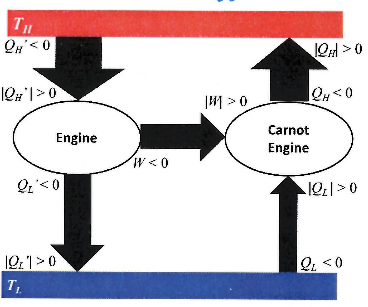
\includegraphics[scale=0.5]{Carnot1.png}
        \vspace{-70pt}
    \end{center}
\end{wrapfigure}

Assume $\eta_{engine} > \eta_{Carnot}$

Run Carnot as a fridge as it is reversible
\begin{gather*}
    \eta = \frac{|W|}{Q_{in}} \\
    \frac{|W|}{|Q_{H}'|} > \frac{|W|}{Q_H} \implies Q_{H} > |Q_{H}'|
\end{gather*}
Use the first law with $dU = 0 ~;~ dU = \delta Q + \delta W$
\begin{gather*}
    \begin{alignedat}{2}
        |Q_{H}'| &+ Q_{L}' = -W     &\quad |W| &+ |Q_{L}| = -Q_{H} \\
        |Q_{H}'| &- |Q_{L}'| = -|W| &\quad |W| &= |Q_H| - |Q_L|
    \end{alignedat} \\
    |Q_{H}'| - |Q_{L}'| = |Q_H| - |Q_L| \\
    |Q_L| - |Q_L'| = |Q_H| - |Q_H'|
\end{gather*}
This is less than zero if the engine is more efficient than a Carnot engine

The net effect is to remove heat from cold to hot with no other change, violating the Clausius Statement of the Second Law

\section{Second Carnot Theorem}
\emph{All reversible engines operating between two reservoirs have the same efficiency}

\begin{wrapfigure}{l}{0.4\textwidth}
    \begin{center}
        \vspace{-20pt}
        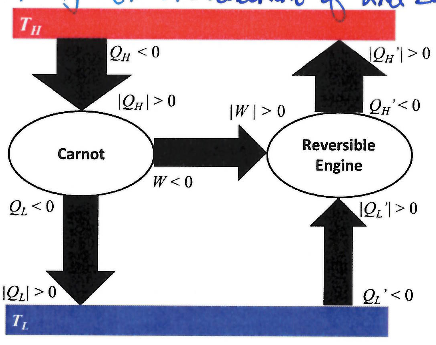
\includegraphics[scale=0.4]{Clausius2.png}
    \end{center}
\end{wrapfigure}

Assume that $\eta_{reversible} < \eta_{Carnot}$

By approaching in a similar way to above, we find that we would transfer a net amount of heat from cold to hot, violating the Clausius statement

\chapter{}
Clausius wanted to understand heat flow in cycles \\
The inequality gives the mathematical description of the Second Law - that processes go in one direction
\begin{equation*}
    \oint \frac{\delta Q_{rev}}{T} \leq 0
\end{equation*}
Consider two engines - one perfect, one not, that take in the same amount of heat, $|Q_H|$ \\
For a reversible Carnot:
\begin{equation*}
    \frac{Q_H}{T_H} = \frac{|Q_L|}{T_L} \implies \frac{Q_{H}}{T_H} - \overbrace{\frac{|Q_L|}{T_L}}^{\text{heat leaving}} = 0 \implies \frac{Q_{H}}{T_H} + \frac{Q_{L}}{T_L} = 0
\end{equation*}
A real engine does less work for the same heat in \\
So $|Q_L'| > |Q_L|$

This engine has lower efficiency so more heat is rejected - $Q_L'$ is more negative
\begin{gather*}
    \frac{Q_{H}}{T_H} + \frac{Q_{L}'}{T_L} < 0 \\
    \oint \frac{\delta Q}{T} \leq 0
\end{gather*}

\begin{wrapfigure}{r}{0.4\textwidth}
    \begin{center}
        \vspace{-30pt}
        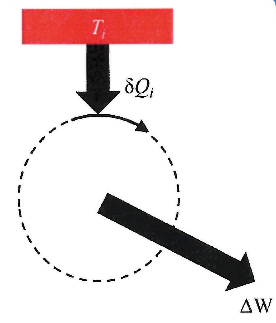
\includegraphics[scale=0.5]{Clausius3.png} \\
        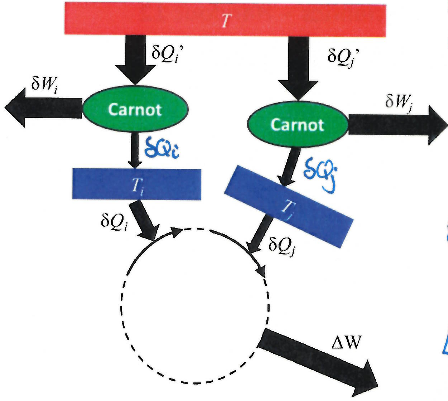
\includegraphics[scale=0.4]{Clausius4.png}
        \vspace{-150pt}
    \end{center}
\end{wrapfigure}

This engine is not quasi-static \\
Heat is added at various points - assume it comes from several heat reservoirs \\
Heat reservoirs have infinite heat capacity and their temperature doesn't change

From the First Law, the engine is cycle so $dU = 0$
\begin{gather*}
    \delta W = -\delta Q \\
    \Delta W_{engine} = \sum \delta Q_i
\end{gather*}
Take heat into the general cycle from that rejected by a number of Carnot engines, which have all got the same hot reservoir
\begin{gather*}
    \delta Q_{i}' = \delta Q_i + \delta W_i \\
    \delta Q_{j}' = \delta Q_j + \delta W_j
\end{gather*}
Add the arrows up \\
 For the Carnot, $\frac{Q_H}{|Q_L|} = \frac{T_H}{T_L} \to \frac{Q_H}{T_H} = \frac{|Q_L|}{T_L}$
 \begin{gather*}
     \frac{\delta Q_i}{T_i} = \frac{\delta Q_{i}'}{T} \\
     \frac{\delta Q_i}{T_i} = \frac{\delta Q_i + \delta W_i}{T} \\
     \delta W_i = T\frac{\delta Q_i}{T_i} - \delta Q_i
 \end{gather*}
The Kelvin statement can't be violated (Second Law) so the engine must do some work, i.e. total work $\leq 0$
\begin{gather*}
    \begin{aligned}
        \text{Total Work } &= \text{Engine Work} + \sum \text{Carnot Work} \leq 0 \\
        &= \Delta W + \sum_{cycle} \delta W_i \leq 0 \\
        &= \cancel{\sum_{cycle} \delta Q_i} + \sum_{cycle} \Big(T\frac{\delta Q_i}{T_i} - \cancel{\delta Q_i} \Big) \leq 0
    \end{aligned} \\
    T\sum_{cycle} \frac{\delta Q_i}{T_i} \leq 0 ~~;~~ T \geq 0 \\
    \begin{aligned}
        \implies & \sum_{cycle} \frac{\delta Q_i}{T_i} \leq 0 \\
        \implies & \oint \frac{\delta Q}{T} \leq 0 ~,~~ \delta Q_i \to 0
    \end{aligned}
\end{gather*}

\section{Entropy}
In Clausius, we had equality for reversible cycles (Carnot), thus $\frac{\delta Q_{rev}}{T}$ is an exact differential
\begin{equation*}
    \oint \frac{\delta Q_{rev}}{T} = 0
\end{equation*}
It doesn't depend on the path so define a function of state, entropy, as
\begin{equation*}
    dS = \frac{\delta Q_{rev}}{T}
\end{equation*}
We can calculate this entropy change between two states:
\begin{equation*}
    dS = \frac{\delta Q_{rev}}{T} \implies S_B - S_A = \int_{A}^{B} dS = \int_{A}^{B} \frac{\delta Q_{rev}}{T}
\end{equation*}
T is always in Kelvin for these integrals

Entropy describes energy quality, i.e. how much work can be got out of a process

The higher the entropy, the 'lower' the temperature; lower temperature reservoirs have less work potential, as the efficiency of an engine between reservoir and environment decreases as temperature of the reservoir approaches the temperature of the environment

Adiabatic processes have $dS = 0$ as $\delta Q_{adiab} = 0$

\subsection{Entropy change in any process}
For any irreversible process between two states, can find a complementary reversible one

Clausius: $\oint \frac{\delta Q}{T} \leq 0$ around a cycle
\begin{gather*}
    \int_{A}^{B} \frac{\delta Q}{T} + \int_{B}^{A} \frac{\delta Q_{rev}}{T} \leq 0 \\
    \int_{A}^{B} \frac{\delta Q}{T} \leq \int_{A}^{B} \frac{\delta Q_{rev}}{T}
\end{gather*}
This will always be true no matter A and B

By definition, $dS = \frac{\delta Q_{rev}}{T}$ so
\begin{equation*}
    \Delta S = \int_{A}^{B} \frac{\delta Q_{rev}}{T} \geq \frac{\delta Q}{T}
\end{equation*}
Adiabatic process has $\delta Q = 0$ so
\begin{equation*}
    \Delta S \geq 0
\end{equation*}
i.e. Entropy always increases

Clausius said that the Universe Entropy tends to a maximum \\
Universe Energy is constant by the First Law

\subsection{Entropy change around a cycle is 0}
Split an arbitrary cycle into a number of smaller Carnot cycles, each interacting with two heat reservoirs \\
Each Carnot has $\oint \frac{\delta Q_{rev}}{T} = 0$

The adiabatic between consecutive Carnots cancel \\
Sum in the limit of Carnots going to zero size:
\begin{equation*}
    \therefore \oint \frac{\delta Q_{rev}}{T} = 0 ~ \text{for any cycle}
\end{equation*}

\subsection{Principle of increase of Entropy}
\emph{In every process taking place in an indeal system, the entropy change of the system either increases of remains constant \\
This is equivalent to Kelvin and Clausius statements}

\begin{wrapfigure}{r}{0.4\textwidth}
    \begin{center}
        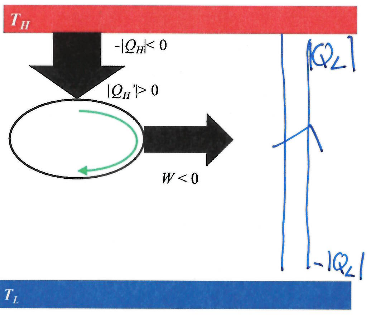
\includegraphics[scale=0.5]{EquivEntropy.png}
    \end{center}
\end{wrapfigure}

Assume we have a Kelvin violator (an engine with no cold sink) \\
$Q_H$ leaves hot so hot reservoir has an entropy change
\begin{equation*}
    \Delta S_H = \int \frac{\delta Q_H}{T_H} = \frac{1}{T_H}\int \delta Q_H = -\frac{|Q_{H}|}{T_H}
\end{equation*}
The engine is a cycle so has no entropy change
\begin{equation*}
    \text{Universe entropy} = 0 - \frac{|Q_{H}|}{T_H} < 0
\end{equation*}
This violates the entropy change

Now look at a Clausius violator:
\begin{itemize}
    \item $-|Q_L|$ leaves cold, entropy change of $-\frac{|Q_L|}{T_L}$
    \item $+|Q_L|$ added to hot, entropy change of $+\frac{|Q_{L}|}{T_H}$
    \item Total entropy change:
            \begin{gather*}
                \Delta S = -\frac{|Q_L|}{T_L} + \frac{|Q_{L}|}{T_H} \\
                \Delta S = |Q_L|\Big(\frac{1}{T_H} - \frac{1}{T_L} \Big) < 0
            \end{gather*}
    \item This violates entropy statement
\end{itemize}

\chapter{}
\begin{wrapfigure}{r}{0.4\textwidth}
    \begin{center}
        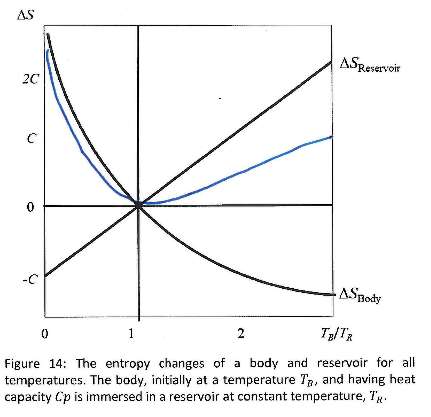
\includegraphics[scale=0.4]{Entropy.png}
        \vspace{-40pt}
    \end{center}
\end{wrapfigure}

Take body of heat capacity $C_p$, temperature $T_B$ \\
Drop it into a water bath (heat reservoir) at $T_R$ and $T_B \to T_R$
\begin{align*}
    \Delta S_{B} &= \int_{T_B}^{T_R} \frac{\delta Q}{T} = \int_{T_B}^{T_R} \frac{C_p \, dT}{T} \\
    \Delta S_{B} &= C_p \ln\Big(\frac{T_R}{T_B}\Big)
\end{align*}
Body takes in (rejects) heat from the reservoir as it comes to equilibrium, correspond to increase (decrease) in its entropy \\
The reservoir energy change is equal and opposite to the body
\begin{align*}
    \Delta Q_{R} &= -\int_{T_B}^{T_R} C_p \, dT \\
                 &= -C_p (T_R - T_B) \\
    \Delta S_{R} &= \int \frac{\delta Q}{T_R} = \frac{\Delta Q_R}{T_R} \\
                 &= -\frac{C_p}{T_R}(T_R - T_B)
\end{align*}
Universe (total) entropy change is
\begin{align*}
    \Delta S_U &= C_p \ln\Big(\frac{T_R}{T_B}\Big) - \frac{C_p}{T_R}(T_R - T_B) \\
               &= C_p \Bigg[\frac{T_B}{T_R} - 1 - \ln\Big(\frac{T_B}{T_R}\Big) \Bigg]
\end{align*}
We can show that $x - 1 - \ln(x) \geq 0 ~\forall ~ x > 0,\, x \neq 1$ \\
Therefore, we have a positive entropy change as $T_R \neq T_B ~;~ T_R, T_B > 0$

\section{Entropy Continued}
If things are left on their own, they tend to a more disordered state.
Energy is required to put them back.
We see that entropy increases naturally.
Perhaps it is better to think about this being related to our increasing knowledge of the system (things become more uncertain)

In the real world, all processes are irreversible, but we can use complementary reversible processes between two thermodynamic states to calculate the lower bound on $\Delta S$ \\
In real processes, there are more ways of converting the system's internal energy to heat, which dissipates into the environment \\
This heat can't be used for work - low quality energy means high entropy

In the example above, we saw that overall entropy increased, but this can be the sum of an increasing and decreasing part \\
Look at the First Law:
\begin{align*}
    dU &= \delta Q + \delta W \\
       &= T\,dS - p\,dV
\end{align*}
This holds for any process \\
If it is irreversible,
\begin{align*}
    T\,dS &\geq \delta Q \\
    -p\,dV &\leq \delta W
\end{align*}
This yields the same result overall

\section{T-S Diagrams}
\begin{wrapfigure}{l}{0.4\textwidth}
    \begin{center}
        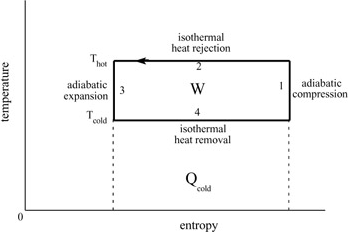
\includegraphics[scale=0.4]{TSDiag.png}
        \vspace{-30pt}
    \end{center}
\end{wrapfigure}

These can be simpler than p-V diagrams

\textit{TS Diagram for a Carnot Cycle on the left}

For an isochoric process:
\begin{equation*}
    \Big(\frac{\p S}{\p T} \Big)_V \to S = \int \Big(\frac{\p S}{\p T} \Big)_V dT
\end{equation*}
Area enclosed:
\begin{equation*}
    \oint T\,dS = \Delta Q \textit{ (net heat)}
\end{equation*}

\section{Thermodynamic Potentials}
Thermodynamic properties are described by functions of state, e.g. $p = p(V,\,T)$, but some are easier to measure than others (pressure is easier than entropy)

We can construct potentials (energies) by adding combinations of variables with dimensions of energy to the U, e.g. TS, pV \\
E.g. For internal energy,
\begin{equation*}
    dU = T\,dS - p\,dV
\end{equation*}
All functions on the right are functions of state (path independent) so this holds for any process. If we change either entropy (dS) or volume (dV), we change U: $U = U(S,V)$ and these are its 'natural variables'

$U = U(S,V)$:
\begin{gather*}
    dU = \Big(\frac{\p U}{\p S}\Big)_V dS + \Big(\frac{\p U}{\p V}\Big)_S dV \\
    T = \Big(\frac{\p U}{\p S}\Big)_V ~;~ p = -\Big(\frac{\p U}{\p V}\Big)_S
\end{gather*}
Can write intensive variables in terms of partial derivatives of extensive ones:
\begin{align*}
    \frac{T}{p} &= -\frac{\big(\tfrac{\p U}{\p S}\big)_V}{\big(\tfrac{\p U}{\p V}\big)_S} \\
    &= -\Big(\frac{\p U}{\p S}\Big)_V \Big(\frac{\p V}{\p U}\Big)_S
\end{align*}
Use the reciprocity theorem:
\begin{gather*}
    \Big(\frac{\p x}{\p y}\Big)_z \Big(\frac{\p y}{\p z}\Big)_x = -\Big(\frac{\p x}{\p z}\Big)_y \\
    \frac{T}{p} = \Big(\frac{\p V}{\p S}\Big)_U
\end{gather*}

\subsection{What is Delta S as an ideal gas expands VA to VB at constant temperature, T0?}
Constant internal energy, $pV = RT_0$
\begin{align*}
    \Delta S &= \int_{A}^{B} \Big(\frac{\p S}{\p V}\Big)_U dV = \int_{V_A}^{V_B} \frac{p}{T_0} = \int_{V_A}^{V_B} \frac{R}{V}dV \\
    &= R\ln\Big(\frac{V_B}{V_A}\Big)
\end{align*}

\section{Enthalpy}
Enthalpy, H, is useful for considering constant pressure processes (open to the atmosphere)

Tends to be much easier to measure and design experiments for

As constant pressure, it behaves like the internal energy would do at constant volume \\
{[}Burning fuel in atmosphere, atmosphere needs pushing out the way; enthalpy takes care of the atmosphere work (invisible){]}

\subsection{Finding Enthalpy}
\begin{align*}
    H &= U + pV \\
    dH &= d(U + pV) = dU + p\,dV + V\,dp \\
    dU &= T\,dS - p\,dV \implies \\
    dH &= T\,dS - \cancel{p\,dV} + \cancel{p\,dV} + V\,dp \\
       &= T\,dS + V\,dp
\end{align*}
Natural variables are entropy and pressure, $H = H(S,p)$

At constant pressure, $dp = 0 \implies dH = T\,dS = \delta Q$
\begin{equation*}
    \delta Q = C_p dT ~\therefore~ \Big(\frac{\p H}{\p T}\Big)_p = C_p = \Big(\frac{\p Q}{\p T}\Big)_p
\end{equation*}
In an isobaric process, the enthalpy is the heat absorbed/rejected

Internal Energy and Enthalpy have Entropy as a natural variable \\
This is diffcult to understand; it is more useful to have temperature

\section{Free Energies}
\begin{align*}
    F &= F(T,V) & G &= G(p, T) \\
    \text{Helmholtz}& \text{ Function} & \text{Gibbs }&\text{Free Energy}
\end{align*}

\subsection{Free Energies}
\begin{align*}
    F &= U - TS \\
    dF &= dU - T\,dS - S\,dT = \overbrace{\cancel{T\,dS} - p\,dV}^{dU = T\,dS - p\,dV} - \cancel{T\,dS} - S\,dT \\
    dF &= -p\,dV - S\,dT
\end{align*}
If temperature is constant, $dT = 0 \implies dF = -p\,dV = \delta W$ \\
Tells us the reversible work done on the surroundings

\chapter{}
\section{Free Energies Continued}
Helmholtz was $F = U - TS$
\begin{align*}
    dF &= -p\,dV - S\,dT \\
    \therefore F &= F(V,T) \\
    dF &= \Big(\frac{\p F}{\p V}\Big)_T dV + \Big(\frac{\p F}{\p T}\Big)_V dT
    ~~\Bigg\{ \begin{aligned}
                -p &= \Big(\frac{\p F}{\p V}\Big)_T \\
                -S &= \Big(\frac{\p F}{\p T}\Big)_V
            \end{aligned}
\end{align*}
At constant temperature, $dT = 0$, so $dF = -p\,dV = \delta W$ \\
Increase Helmholtz, $dF > 0 \implies (F_1 \to F_2 > F_1) \implies \delta W > 0$

The Gibbs function:
\begin{align*}
    G &= U + pV - TS + \underbrace{\cdots}_{\text{Add any other term}} \\
    &= H - TS
\end{align*}
Can show $dG = V\,dP - S\,dT$ so $G = G(P, T)$

There are easiest to manipulate in experiment, the change in G correspond to the max mechanical work \\
If the process is isobaric and isothermal $(dp = dT = 0)$ we have $dG = 0$ \\
The Gibbs function is conserved at phase changes.

\section{Maxwell Relations}
We have seen that thermodynamic functions of state are related to partial derivatives of the potentials. The potentials (U, F, H, G) are functions of state so the order of taking second derivatives doesn't matter. We use this to find ways of relating partial derivatives (changes between two thermodynamic functions) of things that are physically hard to understand to easier ones

\textbf{Proof:}
Consider U:
\begin{align*}
    dU &= T\,ds - p\,dV \\
    &= \Big(\frac{\p U}{\p S}\Big)_V dS + \Big(\frac{\p U}{\p V}\Big)_S dV
\end{align*}
The total differentials are equal:
\begin{equation*}
    T = \Big(\frac{\p U}{\p S}\Big)_V ~;~ -p = \Big(\frac{\p U}{\p V}\Big)_S
\end{equation*}
U is a function of state (exact), $\oint dU = 0$, so
\begin{gather*}
    \Big(\frac{\p^2 U}{\p V \p S}\Big) = \Big(\frac{\p^2 U}{\p S \p V}\Big) \\
    \bigg(\frac{\p}{\p V} \Big(\frac{\p U}{\p S} \Big)_V \bigg)_S = \boxed{\Big(\frac{\p T}{\p V}\Big)_S = -\Big(\frac{\p p}{\p S} \Big)_V} = \bigg(\frac{\p}{\p S} \Big(\frac{\p U}{\p V}\Big)_S \bigg)_V \\
    \Big(\frac{\p T}{\p p}\Big)_S = \Big(\frac{\p V}{\p S}\Big)_p ~;~ \Big(\frac{\p S}{\p V} \Big)_T = \Big(\frac{\p p}{\p T}\Big)_V ~;~ \Big(\frac{\p V}{\p T}\Big)_p = -\Big(\frac{\p S}{\p p} \Big)_T
\end{gather*}

\section{Generalised Quantities}
Some of the derivatives in the Maxwell relations correspond to real physical quantities

Heat capacity is $C = \frac{\Delta Q}{\Delta T}$, but always have on property constant, i.e. $C_V$

We know that $dS = \frac{\delta Q_{rev}}{T}$ and $T\Delta S = \Delta Q$ so
\begin{equation*}
    C = \frac{\Delta Q}{\Delta T} = T\frac{\Delta S}{\Delta T} ~;~ \lim_{\Delta T \to 0} C_{\alpha} = T\Big(\frac{\p S}{\p T}\Big)_{\alpha}
\end{equation*}
Volume expansicity is the fractional volume change with temperature
\begin{equation*}
    \beta_{p} = \frac{dV}{V}\times\frac{1}{\Delta T} \to \beta_{p} = \frac{1}{V} \Big(\frac{\p V}{\p T}\Big)_p ~;~ \beta_S = \frac{1}{V} \Big(\frac{\p V}{\p T}\Big)_S
\end{equation*}
Compressibility: fractional volume change with pressure
\begin{equation*}
    \kappa_T = -\frac{dV}{V} \times \frac{1}{\Delta p} \to \kappa_T = -\frac{1}{V} \Big(\frac{\p V}{\p p}\Big)_T ~;~ \kappa_S = -\frac{1}{V} \Big(\frac{\p V}{\p p}\Big)_S
\end{equation*}
As you increase the pressure on a solud, it gets smaller, so the negative sign gives a positive coefficient

\section{TdS Equations}
Help us to look at material behaviour, $\delta Q = T\,dS$, e.g. heat transfer

\textbf{Proof: Derive TdS by considering $S = S(V,T)$.}
Total differential (multiplied by T):
\begin{equation*}
    T\,dS = T\Big(\frac{\p S}{\p T}\Big)_V dT + T\Big(\frac{\p S}{\p V}\Big)_T dV
\end{equation*}
Recall heat capacity,
\begin{equation*}
    C_V = T\Big(\frac{\p S}{\p T}\Big)_V \text{ - use this as the first term}
\end{equation*}
Now look at the Second Maxwell:
\begin{gather*}
    \Big(\frac{\p S}{\p V}\Big)_T = \Big(\frac{\p p}{\p T}\Big)_V \text{ - use this as second term} \\
    T\,dS = C_V dT + T\Big(\frac{\p p}{\p T}\Big)_V dV
\end{gather*}
If there is no heat input (adiabatic), $\delta Q = T\,dS = 0$
\begin{align*}
    -C_V dT &= T\Big(\frac{\p p}{\p T}\Big)_V dV \\
    -C_V \int \frac{dT}{T} &= \int \Big(\frac{\p p}{\p T}\Big)_V dV
\end{align*}

\section{Energy Equations}
Use the first law to write the internal energy in terms of measurable things
\begin{equation*}
    \Big(\frac{\p U}{\p V}\Big)_T = T\Big(\frac{\p p}{\p T}\Big)_V - p ~;~ \Big(\frac{\p U}{\p p}\Big)_T = -T\Big(\frac{\p V}{\p T}\Big)_p - p\Big(\frac{\p V}{\p p}\Big)_T
\end{equation*}

\textbf{Proof - Derive the 2nd Energy Equation.}
\begin{align*}
    dU &= T\,dS - p\,dV ~~\bigg[\div (dp)_T \\
    \Big(\frac{\p U}{\p p}\Big)_T &= T\Big(\frac{\p S}{\p p}\Big)_T - p\Big(\frac{\p V}{\p p}\Big)_T ~~\bigg[\big(\lim_{\Delta p \to 0}\big)_T
\end{align*}
Use fourth Maxwell relation to simplify:
\begin{gather*}
    \Big(\frac{\p S}{\p p} \Big)_T = -\Big(\frac{\p V}{\p T}\Big)_p \\
    \Big(\frac{\p U}{\p p}\Big)_T = -T\Big(\frac{\p V}{\p T}\Big)_p - p\Big(\frac{\p V}{\p p}\Big)_T
\end{gather*}
To solve problems:
\begin{enumerate}
    \item Write down an appropriate thermodynamic potential
    \item Substitute in Maxwell relations to get nice derivatives
    \item Apply Calculus techniques (reciprocal/reciprocity)
    \item Identify a heat capacity or a generalised quantity
\end{enumerate}

\subsection{General Expression between Cp and CV from kappaT and betap}
\begin{gather*}
    T\,dS = C_V dT + T\Big(\frac{\p p}{\p T}\Big)_V dV ~;~ T\,dS = C_p dT - T\Big(\frac{\p V}{\p T}\Big)_p dp \\
    0 = (C_V - C_p)dT + T \Big(\frac{\p p}{\p T}\Big)_V dV + T\Big(\frac{\p V}{\p T}\Big)_p dp
\end{gather*}
Temperature is a function of state, $T = T(p,V)$
\begin{gather*}
    dT = \Big(\frac{\p T}{\p V}\Big)_p dV + \Big(\frac{\p T}{\p p}\Big)_V dp \\
    (C_p - C_V)\Bigg[\Big(\frac{\p T}{\p V}\Big)_p dV + \Big(\frac{\p T}{\p p}\Big)_V dp \Bigg] = T \Big(\frac{\p p}{\p T}\Big)_V dV + T\Big(\frac{\p V}{\p T}\Big)_p dp
\end{gather*}
The coefficients of dp or dV must be equal on each side:
\begin{equation*}
    (C_p - C_V)\Big(\frac{\p T}{\p p}\Big)_V = T\Big(\frac{\p V}{\p T}\Big)_p
\end{equation*}
Use the reciprocal relation:
\begin{align*}
    \Big(\frac{\p T}{\p p}\Big)_V &\Big(\frac{\p p}{\p T}\Big)_V = 1 \\
    C_p - C_V &= T\Big(\frac{\p V}{\p T}\Big)_p \Big(\frac{\p p}{\p T}\Big)_V
\end{align*}
Now use the reciprocal:
\begin{align*}
    \Big(\frac{\p p}{\p T}\Big)_V &= -\Big(\frac{\p p}{\p V}\Big)_T \Big(\frac{\p V}{\p T}\Big)_p \\
    C_p - C_V &= T\Big(\frac{\p V}{\p T}\Big)_p \Bigg[-\Big(\frac{\p p}{\p V}\Big)_T \Big(\frac{\p V}{\p T}\Big)_p \Bigg] \\
    &= -T\Big(\frac{\p V}{\p T}\Big)_{p}^2 \Big(\frac{\p p}{\p V}\Big)_T
\end{align*}
But
\begin{gather*}
    \beta_p = \frac{1}{V} \Big(\frac{\p V}{\p T}\Big)_{p} ~;~ \kappa_T = -\frac{1}{V} \Big(\frac{\p V}{\p p}\Big)_{T} \\
    \begin{aligned}
        C_p - C_V &= -T[V\beta_p]^2 \times \bigg[\frac{-1}{V\kappa_T}\bigg] \\
        &= + \frac{TV\beta_{p}^2}{\kappa_T}
    \end{aligned}
\end{gather*}

\chapter{}
\section{Energy Equations Continued}
We showed that $C_p - C_V = \frac{TV\beta_{p}^2}{\kappa_T}$, where $\beta_p$ is the expansicity and $\kappa_T$ is the compressibility

$C_p \geq C_V$: $\kappa_T$ is always positive; $\beta_p$ is squared so ignore the sign \\
The heat capacities don't depend on the internal energy \\
As $T \to 0,~ C_p \to C_V$

\subsection{Heat Transfered to VDW gas expanding isothermally at T0}
(VDW - Van Der Waal's)

Use TdS (1)
\begin{equation*}
    T\,dS = C_V dT + T\Big(\frac{\p p}{\p T}\Big)_V dV
\end{equation*}
But heat,
\begin{equation*}
    \delta Q = T\,dS ~;~ p = \frac{RT}{V - b} - \frac{a}{V^2} \to \Big(\frac{\p p}{\p T}\Big)_V = \frac{R}{V - b}
\end{equation*}
We get
\begin{equation*}
    \Delta Q = \int_{V_1}^{V_2} \frac{T_0 R}{V - b}dV = T_0 R\ln\Big(\frac{V_2 - b}{V_1 - b}\Big)
\end{equation*}
The internal energy of an ideal gas doesn't depend on volume

\section{Entropy Applications}
The higher the entropy, the lower the energy quality; you have less potential.
There is more disorder or uncertainty. \\
From the Second Law (Kelvin), we know we must always have a cold reservoir to dump heat.
As the heat goes in it is positive and this leads to an increase in entropy, which is greater than or equal to any negative entropy change elsewhere. \\
The cold sink is thermodynamically the most important.

We know that $\eta = \frac{|Work|}{Heat\,In}$, but how effective is an engine?

Real engines will always do less work than a reversible engine operating between the same two temperatures.
\begin{equation*}
    \eta_{rev} = \frac{|\text{Best Possible Work Out}|}{\text{Heat In}},~ \eta_{rev} \geq \eta
\end{equation*}
We can define effectiveness,
\begin{equation*}
    \eta_{2nd} = \frac{\eta}{\eta_{rev}} = \frac{\text{Actual Efficiency}}{\text{Effectiveness}}
\end{equation*}

\section{Availability and Available Energy}
We want to know what is the maximum work we can theoretically achieve in a process.
Here for max work, use reversible cycles (Carnot) to take all the heat from the start to finish and the process ends in a dead state, a state in thermal equilibrium with the environment.

Availability:
\begin{gather*}
    A = U + \underbrace{p_0 V}_{\text{Work against env}} - \underbrace{T_0 S}_{\text{Env entropy change}} \\
    dA = dU + p_0 (V_2 - V_1) - T_0 (S_2 - S_1)
\end{gather*}
Consider an infinitesimal amount of heat taken into the system from the environment at constant volume and temperature \\
If the environment (surroundings) are at $T_0$, $dS_{env} = -\frac{\delta Q}{T_0}$ \\
Negative entropy as heat comes out of surroundings
\begin{equation*}
    \Delta S_U = dS_{system} + dS_{env} = dS_{system} - \frac{\delta Q}{T_0} \geq 0
\end{equation*}
As the system exchanges heats with its surroundings, it does work/has work done on it \\
Energy is conserved, look at First Law: $dU = \delta Q + \delta W$ \\
The work is:
\begin{align*}
    \delta W &= \delta W_{system} - \underbrace{p_0 dV}_{\text{Work on env, cst p}} \\
    \delta W_{system} &= dU + p_0 dV - \delta Q \\
    &\geq dU + p_0 dV - T_0 dS_{system} ~[\delta Q \leq T_0 dS_{system}] \\
    \delta W_{system} &\geq dA
\end{align*}
In other words, the change in availability provides the energy for doing work \\
If the system is mechanically isolated, $\delta W_{system} = 0$, so $dA = (A_{f} - A_{i}) \leq 0$
\begin{equation*}
    \delta W = dU - \delta Q \geq dU - T_0 dS_{system} = d(U - T_0 S)
\end{equation*}
Recall $F = U - TS$: $\implies \delta W \geq dF$ at constant T \\
i.e. Work Done $\geq$ Change in Helmholtz function

The Helmholtz and Gibbs functions, changes in which don't depend on entropy change, will tell us how much can be done and if a process is spontaneous

\subsection{Express Delta S(env) in terms of U}
The pressure is constant so,
\begin{align*}
    dU &= \delta Q - p_0 dV \\
    &= \delta Q,~ dV = 0
\end{align*}
If $dV = 0$ at $T_0$ for environment temperature:
\begin{align*}
    \Delta S_{env} &= -\frac{\Delta Q}{T_0} = -\frac{\Delta U}{T_0} \\
    \Delta S_{U} &= \Delta S_{system} + \Delta S_{env} = \Delta S_{system} - \frac{\Delta U}{T_0} \\
    T_0 \Delta S_U &= T_0\Delta S_{system} - \Delta U \\
    -T_0 \Delta S_U &= \Delta U - T_0\Delta S_{system}
\end{align*}
Now $F = U - T_0 S$ at constant T, so $\Delta F = \Delta U - T_0 \Delta S$

The two right hand sides are identical \\
The Helmholtz function is a 'disguised form' of the entropy change of the Universe at constant temperature and volume.

If $\Delta S_U$ spontaneously increase, $\Delta F$ must decrease \\
So if we minimise F, we get the most work out and the system reaches equilibrium

$T_0 dS$ is really the energy the system provides to the surroundings as it does work.
The environement entropy increases to compensate for the system energy decrease

The Gibbbs function does the same job at constant pressure
\begin{equation*}
    dG = dU - T_0 dS + p_0 dV = dA,~ dp = dT = 0
\end{equation*}

\section{Useful Work and Irreversibility}
\begin{equation*}
    I = |W_{rev} - W_{use}| = T_0 \Delta S_U
\end{equation*}
$W_{rev}$ is work a reversible device does (Carnot)
\begin{equation*}
    W_{use} = W_{actual} - W_{env}
\end{equation*}
In any real device, some work is done pushing the surroundings out of the way.

\chapter{}
\section{Irreversibility Continued}
$W_{rev}$ - Work a totally reversible (perfect) device does operating between two temperatures \\
Useful work, $W_{use}$ - Work any device does that can be used for motion (i.e. not against the environment)
\begin{align*}
    W_{use} &= \underbrace{W_{actual}}_{\text{Work produced}} - \underbrace{W_{env}}_{\text{Work done on env}} \\
    \text{Irreversibility, }I &= |W_{rev} - W_{use}| = T_0 \Delta S_U
\end{align*}
$T_0$ in this case is the \textit{lowest available reservoir}

\subsection{Heat is supplied from a furnace to an ideal gas in a piston}
Volume doubles at constant $T_0$
\begin{figure}[H]
    \centering
    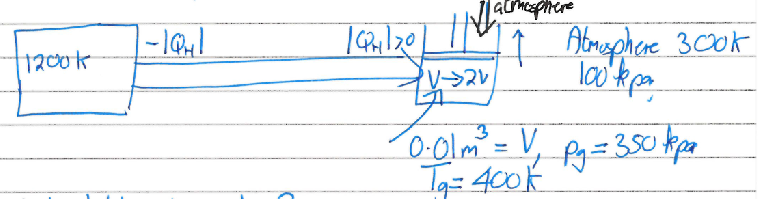
\includegraphics[scale=0.5]{Ex132.png}
\end{figure}
a) What is the total work gas does?
\begin{align*}
    \Delta W_{piston} &= \int_{V}^{2V} -p\,dV ~~[nrT_g = pV] \\
    &= \int_{V}^{2V} -\frac{nrT_g}{V}dV \\
    &= -nrT_g \ln2 = -350\,kpa \times 0.01\,m^3\,\ln2 \\
    &= -2.43\,kJ
\end{align*}
b) What is the atmosphere work?
\begin{align*}
    W_{env} &= \int_{V}^{2V} -p_{atm}dV = -p_{atm} \times V = -1.00\,kJ \\
    W_{use} &= W_{piston} - W_{env} = -1.43\,kJ
\end{align*}
c) What is the irreversibility of this process? \\
Heat hasn't been moved using reversible engines

All the heat from the furnace is used to expand gas as work \\
For gas, $dU = 0$ (isothermal) so from $dU = \delta Q + \delta W$,
\begin{equation*}
    W_{gas} = W_{piston} = -|Q_H|
\end{equation*}
Furnace entropy:
\begin{align*}
    \Delta S_{furnace} &= -\frac{|Q_H|}{T_{furnace}} \\
    &= -\frac{2.43\,kJ}{1200\,K} = -2.03\,J\,K^{-1}
\end{align*}
Gas:
\begin{align*}
    \Delta S_{gas} &= +\frac{|Q_H|}{T_{gas}} \\
    &= \frac{2.43\,kJ}{400\,K} = +6.07\,J\,K^{-1} \\
    \Delta S_U &= +4.05\,J\,K^{-1} \\
    I &= T_0 \Delta S_U = 1.21\,kJ
\end{align*}

\begin{wrapfigure}{r}{0.4\textwidth}
    \begin{center}
        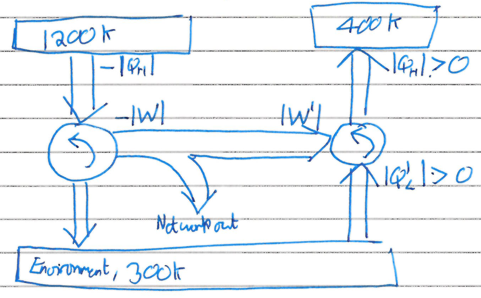
\includegraphics[scale=0.4]{Carnot10.png}
        \vspace{-50pt}
    \end{center}
\end{wrapfigure}
Connect this with Carnot cycles: \\
Engine takes in 2.43 kJ from furnace - $|Q_H| = 2.43\,kJ$
\begin{align*}
    \eta &= 1 - \frac{T_L}{T_H} = \frac{|Work|}{Heat\,In} \\
    \therefore |W| &= Q_H \Big(1 - \frac{300}{1200}\Big) = (-)1.83\,kJ
\end{align*}
Some of the work drives a heat pump that takes $|Q_H|$ to the gas
\begin{gather*}
    CoP_H = \frac{Q_H}{Work} = \frac{T_{gas}}{T_{gas} - T_0} = \frac{400}{400 - 300} = 4 \\
    W' = \frac{Q_H}{4} = 0.61\,kJ \\
    \Delta W = W + W' = -1.82 + 0.61 = -1.21\,kJ
\end{gather*}
1.21 kJ of work potential from the heat of the furnace has been 'lost' in the original transfer of heat to the gas expansion
\begin{equation*}
    W_{rev} = W_{use} + W_{engine} + W_{pump} = -1.43 - 1.82 + 0.61 = -2.64\,kJ
\end{equation*}

\section{Heat Engines and Fridges}
Should be able to sketch any engine cycle given a good starting point (thermo processes) to calculate efficiency. In general, engines:
\begin{itemize}
    \item[-] take in heat from a hot reservoir
    \item[-] do some work (expanding gas) using a working fluid
    \item[-] reject waste heat at low temperature
    \item[-] return engine to original state
\end{itemize}
\begin{align*}
    \eta = \frac{Product}{Expense} \implies& \eta_{engine} = \frac{|Work|}{Heat\,In} = 1 - \frac{|Q_L|}{Q_H} = 1 - \frac{T_L}{T_H} \\
    & CoP_L = \frac{Heat\,from\,cold}{Work} = \frac{|Q_L|}{Q_H - |Q_L|} = \frac{T_L}{T_H - T_L} \\
    & CoP_H = \frac{Heat\,to\,hot}{Work} = \frac{Q_H}{Q_H - |Q_L|} = \frac{T_H}{T_H - T_L}
\end{align*}
Model real if the complexities are manageable \\
In workshop 2, we showed that the adiabatic works cancelled for a Carnot cycle, so the total work was the difference in the isotherm works. Constructing isothermal heat transfer is diffcult - takes a long time to complete.

In practice, construct engines that are only internally reversible. \\
Constructed a cycle from reversible processes, but the heat is added across a temperature difference.

If add heat isochorically (isobarically):
\begin{equation*}
    Q = \int_{T_L}^{T_H} C\,dT
\end{equation*}
for heat $\delta Q$, temperature rise is dT \\
Heat is added quickly from $T_L \to T_H$

Could replace ideal gas with a vapour (changes phase around cycle). Can use open engines (when the working fluid is replaced each cycle) as opposed to closed engines (retain the working fluid and put it back to its initial state at the end of the cycle)

Internal combustion engines - burn fluid in engine \\
External combustion engines - supply heat from external source
\begin{figure}[H]
    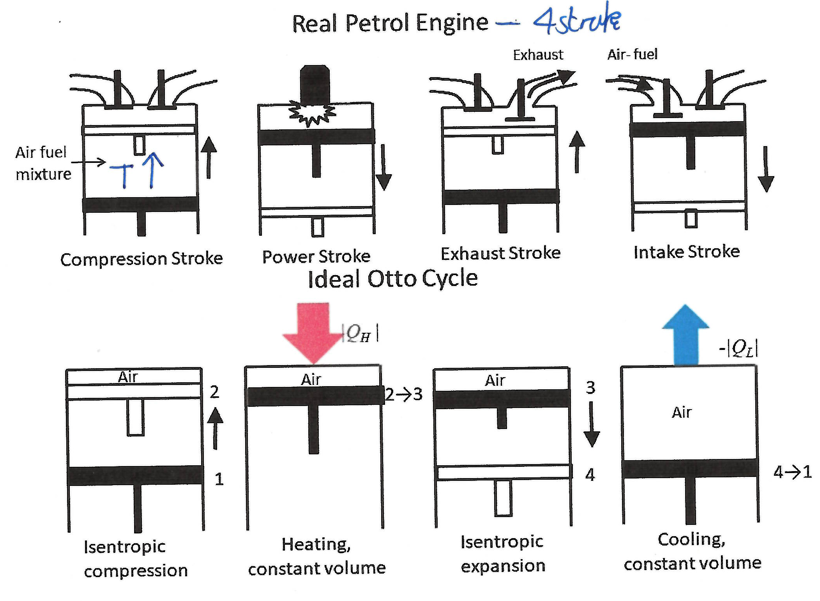
\includegraphics[scale=0.5]{Petril.png}
\end{figure}

\chapter{}
Gas cycles are modelled using 'air standard' assumptions - to make things simple we have an enclosed ideal gas as the working fluid, heat added from external source.
No exhaust - constant volume heat rejection. \\
The 4-stroke petrol engine can be modelled by the Otto cycle using internally reversible processes.
This is similar to the Diesel cycle.
In both cases, only internally reversible as adding heat isochorically/isobarically $[\Delta Q = \int C_V dT]$ - quickly added across temperature difference. \\
Efficiency is lower than for totally reversible (Carnot) cycle between same two temperatures, isothermal heat interactions. \\
The Stirling and Ericsson cycles have same efficiency as a Carnot cycle.
They use regeneration where isochoric/isobaric heat doesn't leave the confines of the engine.

\section{The Otto (Petrol) Cycle}
\begin{wrapfigure}{r}{0.4\textwidth}
    \begin{center}
        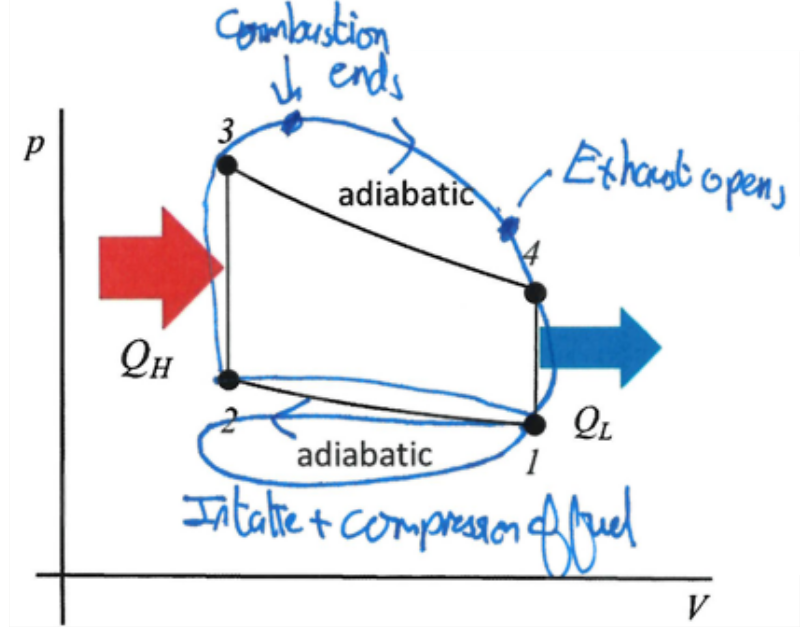
\includegraphics[scale=0.2]{Otto.png}
        \vspace{-200pt}
    \end{center}
\end{wrapfigure}
\begin{align*}
    \eta_{Otto} &= 1 - \frac{T_4 - T_1}{T_3 - T_2} = 1 - \Big(\frac{V_1}{V_2}\Big)^{1 - \gamma} \\
    &= 1 - r^{1 - \gamma} \\
    \eta &= \frac{|Work|}{Heat\,In} = \frac{|Q_H - |Q_L||}{Q_H}
\end{align*}
\begin{itemize}
    \item[1-2:] Adiabatic compression, $Q_{12} = 0$
                \begin{align*}
                    p_1 V_{1}^\gamma &= p_2 V_{2}^\gamma = k_1 \\
                    p_1 V_{1} &= RT_1 \\
                    T_1 V_{1}^{\gamma - 1} &= T_2 V_{2}^{\gamma - 1}
                \end{align*}
    \item[2-3:]  Isochoric heating
                \begin{equation*}
                    Q_H = \int_{T_2}^{T_3} C_V dT = C_V (T_3 - T_2)
                \end{equation*}
    \item[3-4:] Adiabatic compression, $Q_{34} = 0$
                \begin{equation*}
                    T_3 V_{3}^{\gamma - 1} = T_4 V_{4}^{\gamma - 1} = k_2
                \end{equation*}
    \item[4-1:] Isochoric cooling
                \begin{equation*}
                    Q_L = C_V (T_1 - T_4) < 0
                \end{equation*}
\end{itemize}
\begin{equation*}
    \eta = \frac{C_V (T_3 - T_2) - C_V (T_4 - T_1)}{C_V (T_3 - T_2)} = 1 - \frac{T_4 - T_1}{T_3 - T_2} = 1 - \frac{T_1 \cancel{\big(\tfrac{T_4}{T_1} - 1\big)}}{T_2 \cancel{\big(\tfrac{T_3}{T_2} - 1\big)}}
\end{equation*}
Use adiabatics to prove cancelling:
\begin{gather*}
    T_1 V_{1}^{\gamma - 1} = T_2 V_{2}^{\gamma - 1} ~;~ T_3 V_{3}^{\gamma - 1} = T_4 V_{4}^{\gamma - 1} \\
    \frac{T_1}{T_2} = \frac{V_{2}^{\gamma - 1}}{V_{1}^{\gamma - 1}} = \frac{T_4}{T_3}  \implies \frac{T_4}{T_1} = \frac{T_3}{T_2}
\end{gather*}
Now calculate efficiency with the compression ratio, $r = \frac{V_1}{V_2}$
\begin{align*}
    \eta &= 1 - \frac{T_1}{T_2} = 1 - \Big(\frac{V_2}{V_1}\Big)^{\gamma - 1} \\
    &= 1 - r^{1 - \gamma}
\end{align*}
r is typically between 7 and 10 so $\eta \approx 30\%$

\newpage
\section{The Diesel Cycle}
\begin{wrapfigure}{r}{0.4\textwidth}
    \begin{center}
        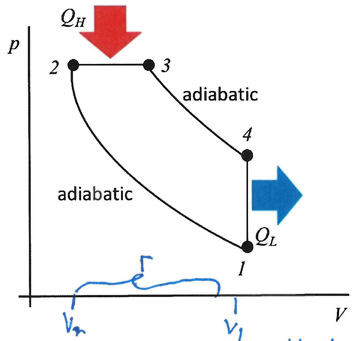
\includegraphics[scale=0.5]{Diesel.png}
        \vspace{-300pt}
    \end{center}
\end{wrapfigure}

\begin{equation*}
    \eta_{Diesel} = 1 - \frac{1}{r^{\gamma - 1}} \Bigg[\frac{r_{c}^\gamma - 1}{\gamma (r_c - 1)}\Bigg]
\end{equation*}
Heat is added at constant pressure:
\begin{gather*}
    r = \frac{V_1}{V_2}, ~\text{ compression ratio} \\
    r_c = \frac{V_3}{V_2}, ~\text{ cut off ratio}
\end{gather*}
Heat added to a pressurised gas \\
If $r_c = 1$, $\eta_{Diesel} \to \eta_{Otto}$, otherwise for any r,
\begin{equation*}
    \eta_{Diesel} > \eta_{Otto}
\end{equation*}
This is useful for high power applications
\begin{figure}[H]
    \centering
    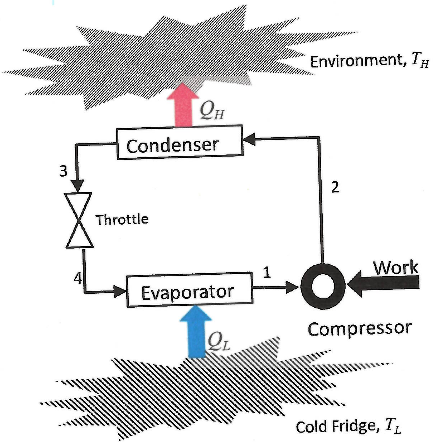
\includegraphics[scale=0.5]{Throttle.png}
    \hspace{20pt}
    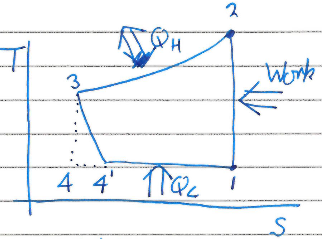
\includegraphics[scale=0.7]{Throttle2.png}
\end{figure}
\begin{itemize}
    \item[1-2:] Adiabatic compression (work supplied)
    \item[2-3:] Isobaric heat rejection (gas is hotter than the atmosphere)
    \item[3-4:] Throttle in expansion device (cools gas to lower than the fridge)
    \item[4-1:] Isobaric and Isothermal heat absorption
\end{itemize}
\begin{equation*}
    \Delta Q = \int T\,dS
\end{equation*}
Larger area enclosed (i.e. 4 not 4') - more heat absorbed \\
In practice, 3-4 (adiabatic expansion) is hard

\section{Phases of a Substance}
Phase changes are fascinating. A small change in one property (e.g. temperature) can lead to a large change in another (volume) as cross phases boundary liquid to gas. \\
At the transition, the phases coexist, but must be at equilibrium with respect to the particle charge. \\
Look at the Gibbs function:
\begin{align*}
    G &= U + pV = TS \\
    dG &= V\,dp - S\,dT
\end{align*}
At the actual phase boundary, $dp = dT = 0 \to dG = 0$ \\
$dG \leq dA$ so we minimise G for equilibrium
\begin{figure}[H]
    \centering
    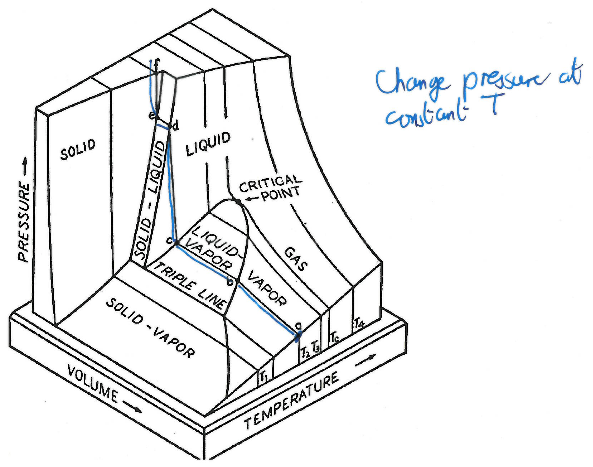
\includegraphics[scale=0.5]{Phases.png}
\end{figure}
Until a, the substance is a gas \\
ab - substance becomes a vapour (temperature lower than its critical temperature)

At b, the substance separates into two phases (liquid and gas) having the same temperature and pressure. The liquid and gas occupy different volumes as they have different densities.

At c, all of the material is in liquid phase, until d, when the solid begins to separate out. \\
de - this is constant pressure freezing

Above e, all the material is a solid. This curve is very steep as increasing the pressure hardly changes its volume.

\section{Phases Transitions and Gibbs}
\begin{wrapfigure}{l}{0.4\textwidth}
    \begin{center}
        \vspace{-30pt}
        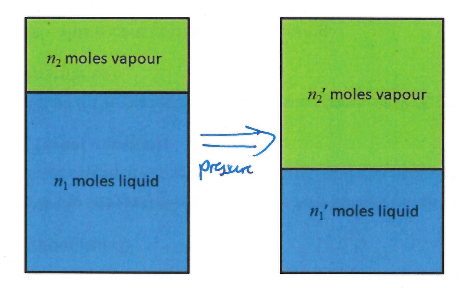
\includegraphics[scale=0.4]{GibbsPhase.png}
        \vspace{-100pt}
    \end{center}
\end{wrapfigure}
The Gibbs function in each phase must be equal
\begin{align*}
    \text{Liquid} &= \begin{cases} g_1 & \text{before} \\ g_1 & \text{after} \end{cases} \\
    \text{Vapour} &= \begin{cases} g_2 & \text{before} \\ g_2 & \text{after} \end{cases} \\
    \text{Specific Gibbs, }& g = \frac{G}{n}
\end{align*}
\begin{gather*}
    N = n_1 + n_2 = n_{1}' + n_{2}' \\
    G = n_1 g_1 + n_2 g_2 ~;~ G' = n_{1}' g_{1}' + n_{2}' g_{2}' \\
    dG = V\,dp - S\,dT,\, dp = dT = 0 \\
    dG = G' - G \to G' = G \\
    n_1 g_1 + n_2 g_2 = n_{1}' g_{1}' + n_{2}' g_{2}'
\end{gather*}
This holds for all $n \iff g_{1}' = g_{2}' ~\&~ g_1 = g_2$
\begin{equation*}
    (n_1 + n_2)g = (n_{1}' + n_{2}')g' \implies g = g'
\end{equation*}
Specific Gibbs is the same in each phase, but the derivative may be different
\begin{figure}[H]
    \centering
    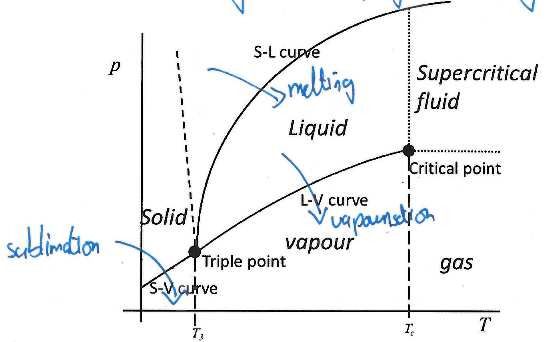
\includegraphics[scale=0.5]{Phasez.png}
\end{figure}

\chapter{}
The Gibbs function takes the same value in each phase (continuous) \\
However, the derivatives might not (slopes aren't smooth)

To change phase, we add latent heat, $L = \Delta Q_{rev}$ \\
But the temperature is constant:
\begin{align*}
    \delta Q_{rev} &= T_0 dS \\
    \Delta Q_{rev} &= L = \int T_0 dS = T_0 (S_2 - S_1)
\end{align*}
Entropy change between phases if latent heat added

\section{Phase Boundary}
We have temperature change, dT, between phases, and $dp = 0$
\begin{gather*}
    G = U + pV - TS ~;~ dG = -S\,dT + V\,dp \\
    dp = 0 \implies dG = -S\,dT \\
    \Big(\frac{\p G}{\p T}\Big)_p = -S
\end{gather*}
So:
\begin{align*}
    \Big(\frac{\p G_1}{\p T}\Big)_p &\neq \Big(\frac{\p G_2}{\p T}\Big)_p \\
    S_1 &\neq S_2
\end{align*}
We have entropy change on going from phase 1 to phase 2
\begin{align*}
    \Delta S &= S_2 - S_1 \neq = 0 \\
    \implies L &= T_0 (S_2 - S_1)
\end{align*}
Take second derivatives:
\begin{equation*}
    \Big(\frac{\p^2 G}{\p T^2}\Big) = \Bigg(\frac{\p}{\p T}\Big(\frac{\p G}{\p T}\Big)_p\Bigg) = -\Big(\frac{\p S}{\p T}\Big)_p
\end{equation*}
General heat capacity is
\begin{equation*}
    C_\alpha = T\Big(\frac{\p S}{\p T}\Big)_\alpha \implies \Big(\frac{\p^2 G}{\p T^2}\Big) = -\frac{C_p}{T}
\end{equation*}
So if discontinuous second derivatives have discontinuity in the heat capacity:

\section{Clausius-Clapyeron Equation}
What is the slope of the equilibrium line in the pT plane between two phases i and f?

Slope is the gradients:
\begin{equation*}
    \Big(\frac{\p p}{\p T}\Big)_{i \to f} = \frac{L_{i \to f}}{T(V_f - V_i)}
\end{equation*}
$V_f$ is volume in final state, $V_i$ is initial volume, $L_{i \to f}$ is the latent heat between states i and f
\begin{equation*}
    T\,dS = C_V dT + T\Big(\frac{\p p}{\p T}\Big)_V dV
\end{equation*}
Consider phase change isothermally, $dT = 0$:
\begin{align*}
    T_0 dS &= T_0 \Big(\frac{\p p}{\p T}\Big)_V dV \\
    T_0 (S_f - S_i) &= T_0 \Big(\frac{\p p}{\p T}\Big)_{i \to f} (V_f - V_i) \\
    [L &= T_0 (S_f - S_i)] \\
    \Big(\frac{\p p}{\p T}\Big)_{i \to f} &= \frac{L_{i \to f}}{T(V_f - V_i)}
\end{align*}

\section{Low Temperatures}
Many interesting and remarkable effects appear at low temperatures (Bose-Einstein condensation, superfluidity, etc) \\
Need low temperatures for CERN, MRI scanners, etc \\
How do we get to low temperatures? Expand a gas.

Joule Expansion:
\begin{equation*}
    \Big(\frac{\p T}{\p V}\Big)_U \iff \Big(\frac{\text{Change in temp}}{\text{Given change in volume}}\Big)_{\text{Internal energy}}
\end{equation*}
$U = U(T)$ so have $\Delta T = 0$. Gases with 'real' behaviour cool, but only by a small amount. \\
Joule-Kelvin - constant enthalpy

\section{Joule-Kelvin Effect}
\begin{wrapfigure}{l}{0.4\textwidth}
    \begin{center}
        \vspace{-20pt}
        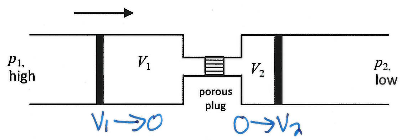
\includegraphics[scale=0.45]{JouleKelvin1.png}
        \vspace{-40pt}
    \end{center}
\end{wrapfigure}

Gas expands through a plug \\
Force gas through from left (do work) $W_L = p_1 V_1$

Gas on right does work, pushing on the piston, $W_R = -p_2 V_2$
No heat exchange, $\delta Q = 0$ and $dU = \delta W$ (First Law)

\begin{align*}
    U_2 - U_1 &= W_L + W_R \\
    &= p_1 V_1 - p_2 V_2 \\
    \implies U_2 + p_2 V_2 &= U_1 + p_1 V_1
\end{align*}
Enthalpy, $H = U + pV$, hence $H_2 = H_1$ and $dH = 0$ \\
Joule-Kelvin cooling is constant enthalpy
\begin{equation*}
    dH = T\,dS + V\,dp
\end{equation*}
So $H = H(S,p)$, also $H = H(T,p)$ \\
Divide dH by dp at constant T:
\begin{align*}
    \Big(\frac{\p H}{\p p}\Big)_T &= T\Big(\frac{\p S}{\p p}\Big)_T + V \\
    \Big(\frac{\p S}{\p p}\Big)_T &= -\Big(\frac{\p V}{\p T}\Big)_p \\
    \Big(\frac{\p H}{\p p}\Big)_T &= V - T\Big(\frac{\p V}{\p T}\Big)_p
\end{align*}

\begin{wrapfigure}{l}{0.4\textwidth}
    \begin{center}
        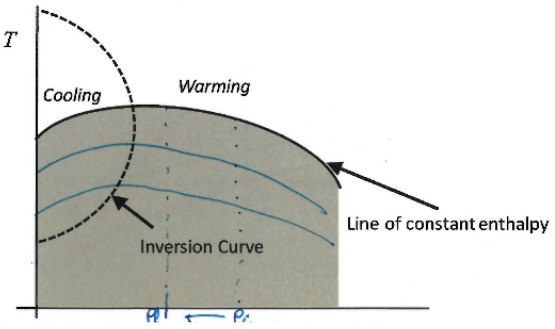
\includegraphics[width=0.4\textwidth]{JouleKelvin2.png}
        \vspace{-50pt}
    \end{center}
\end{wrapfigure}

How does pressure change the temperature? \\
Take partial derivatives at constant enthalpy:
\begin{equation*}
    \Big(\frac{\p T}{\p p}\Big)_H = -\Big(\frac{\p T}{\p H}\Big)_p \Big(\frac{\p H}{\p p}\Big)_T
\end{equation*}
Enthalpy is like U at constant pressure, so
\begin{align*}
    C_p &= \Big(\frac{\p H}{\p T}\Big)_p \\
    \mu_{JK} &= \Big(\frac{\p T}{\p p}\Big)_H = -\frac{1}{C_p} \bigg[V - T\Big(\frac{\p V}{\p T}\Big)_p\bigg] \\
    \Delta T &= \int \mu_{JK} dp
\end{align*}
Expand gas $p_i \to p_f$ with $p_f < p_i$ \\
Joule-Kelvin cools gas if below the inversion temperature \\
To get to the inversion temperature, can adiabatically expand \\
Always cause cooling, but the lower the starting temperature, the lower the temperature reduction

\section{Adiabatic Expansion}
\begin{wrapfigure}{l}{0.4\textwidth}
    \begin{center}
        \vspace{-30pt}
        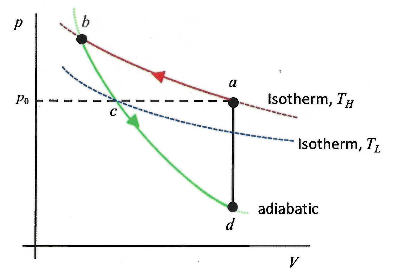
\includegraphics[width=0.4\textwidth]{AdiExp.png}
        \vspace{-70pt}
    \end{center}
\end{wrapfigure}

Compress isothermally ab \\
Adiabatic expansion, bc
\begin{equation*}
    p_c = p_a = p_0
\end{equation*}
Adiabatic is steeper, on a low temperature isotherm

Once at 4.2 K, can't cool by expansion

Pump on the Helium use dilution refrigeration, gives mK ($10^-3$ K)

\section{Adiabatic (De)magnetisation}
\begin{wrapfigure}{l}{0.4\textwidth}
    \begin{center}
        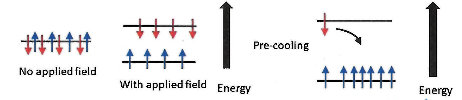
\includegraphics[width=0.4\textwidth]{Magnets1.png} \\
        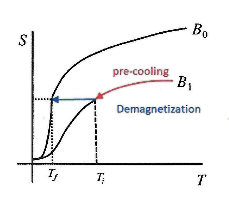
\includegraphics[width=0.4\textwidth]{Magnets2.png}
    \end{center}
\end{wrapfigure}

Surround sample with metal plates, pre-cool in an applied field to mK

in the field, the spins order and spin up is more energetically favourable \\
Pre-cooling means most spins align with the field (high order)

Thermally decouple and adiabatically demagnetise \\
Spin alignment becomes random

Spin entropy has increased. No overall entropy change, so molecule entropy decreases by the same amount (molecules hold electron spin) \\
More ordered molecules $\implies$ lower temperature

\chapter{}
\section{The Third Law of Thermodynamics}
The Second Law tells us about entropy change between states:
\begin{equation*}
    C_p = T\Big(\frac{\p S}{\p T}\Big)_p
\end{equation*}
Separate variables and integrate:
\begin{align*}
    \Delta S &= \int_{T_A}^{T_B} \frac{C_p dT}{T} \\
    &= S_B - S_A = S(T_0) + \int_{T_0}^{T_f} \frac{C_p dT}{T}
\end{align*}
What is $S(T_0)$?
\begin{itemize}
    \item[-] We can define this statiscally using $S = k_B \ln(\Omega)$
    \item[-] Define at a fixed temperature, $S(T = 0)$
\end{itemize}
Nernst examined experimental data:
\begin{align*}
    \Delta H &> 0 \text{ - exothermic} \\
    \Delta H &< 0 \text{ - endothermic}
\end{align*}
Enthalpy, $H = U + pV$ so $dH = T\,dS + V\,dp$ so at constant pressure, $dp = 0$, and $dH = T\,dS = \delta Q$

In nature, minimise Gibbs function for maximum non-mechanical work, at equilibrium:
\begin{align*}
    \Delta G &= G_2 - G_1 < 0 \text{ - spontaneous process} \\
    G &= U + pV - TS \\
    \Delta G &= \Delta U + V_0 \Delta p - T_0 \Delta S
\end{align*}
Maximising $\Delta S$ minimises $\Delta G$
\begin{align*}
    G &= H - TS \\
    \Delta G &= \Delta H - T_0 \Delta S
\end{align*}

\begin{wrapfigure}{l}{0.4\textwidth}
    \begin{center}
        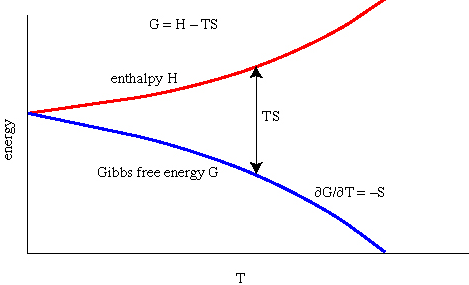
\includegraphics[scale=0.4]{G-H.png}
        \vspace{-30pt}
    \end{center}
\end{wrapfigure}

Nernst noted that $\Delta G$ tends to $\Delta H$ asymptotically as you reach lower temperatures and approach absolute zero

He also proposed that the rates of the changes of G and H tend to zero:
\begin{equation*}
    \lim_{T \to 0} \Big(\frac{\p \Delta G}{\p T}\Big)_p = 0 = \lim_{T \to 0} \Big(\frac{\p \Delta H}{\p T}\Big)_p
\end{equation*}
Total derivative of Gibbs is
\begin{align*}
    dG &= -S\,dT + V\,dp \\
    \implies & \Big(\frac{\p G}{\p T}\Big)_p = -S
\end{align*}
As $\Delta G \to \Delta H$ as $T \to 0$:
\begin{align*}
    \lim_{T \to 0} T\Big(\frac{\p \Delta G}{\p T}\Big)_p = 0 &= \lim_{T \to 0} \Bigg[\Big(\frac{\p G_2}{\p T}\Big)_p - \Big(\frac{\p G_1}{\p T}\Big)\Bigg] \\
    &= -\lim_{T \to 0}[S_2 - S_1]
\end{align*}
Neat to absolute zero, the entropy change of any reaction in a system (in internal equilibrium) is zero

Planck strengthened this to: \\
\emph{"The entropy change of all systems in internal equilibrium is the same at absolute zero, and may be taken to be zero"}

Simon further considered the individual components of a system and how they contribute to the entropy (electrons, spins, etc) \\
We just look at the component of entropy we're interested in, it will be zero

The Third Law has consequences:
\begin{itemize}
    \item Heat capacities tend to zero as $T \to 0$
    \item Thermal expansion stops
    \item Gases do not remain ideal
\end{itemize}

\subsection{Adiabatic Volume Change, V1 to V2 > V1}
Work must be done (negative) as expansion
\begin{align*}
    dU &= \delta Q + \delta W, ~~[\delta Q = 0 \\
    &= \delta W \\
    U_2 - U_1 &= -\int p\,dV < 0 \\
    U_2 < U_1 &\implies T_2 < T_1
\end{align*}
Near $T = 0$K, entropy $\approx 0 \implies S = S(V, T)$
\begin{align*}
    \Delta S &= \int_{0}^{T} \frac{C_V dT}{T},~~ T_i \to T_f,\,T_i \to T_2 \\
    \Delta S_1 = \int_{T_i}^{T_1} \frac{C_V dT}{T} &= \Delta S_2 = \int_{T_i}^{T_2} \frac{C_v dT}{T}
\end{align*}
If we keep expanding the gas, $T_2 \to 0$ and $\Delta S_2 = 0$, but if $C_V > 0$ and $T_1 > 0$, $\Delta S_1 \neq 0$ so we have a contradiction unless you can't get to $T = 0$K

This leads to another statement of the Third Law: \emph{We can't get to $T = 0$K}

\section{Thermodynamics In Action}
As per Week 6's problem class, can look at thermodynamics of many other systems if:
\begin{itemize}
    \item The potential $pV$ is changed to $Xx$
    \item The work does $-p\,dV$ goes to $X\,dx$
\end{itemize}
$X$ is generalised force \\
$x$ is generalised displacement
\begin{equation*}
    \delta W: -p\,dV \to +f\,dx
\end{equation*}

\subsection{A Rod Placed Under Tension}
Rod of area $A$, and length $x$ is placed under tension, $f$, causing $dx$ extension at constant T

Young's Modulus:
\begin{align*}
    E_T &= \frac{Stress}{Strain} \\
    Stress &= \frac{df}{A} ~;~ Strain = \frac{dx}{x} \\
    E_T &= \frac{df}{A} \div \frac{dx}{x} = \frac{x}{A} \Big(\frac{df}{dx}\Big)_T
\end{align*}
How does the tension change with temperature at constant length?
\begin{align*}
    \Big(\frac{\p f}{\p T}\Big)_x &= -\Big(\frac{\p f}{\p x}\Big)_T \Big(\frac{\p x}{\p T}\Big)_f \\
    \Big(\frac{\p f}{\p T}\Big)_x &= -\frac{AE_T}{x}\Big(\frac{\p x}{\p T}\Big)_f,~ \underbrace{\alpha_f = \frac{1}{x}\Big(\frac{\p x}{\p T}\Big)_f}_{\text{Expansicity - }\beta_p}
\end{align*}
The sign of $\Big(\frac{\p f}{\p T}\Big)_x$ depends on the sign of $\Big(\frac{\p x}{\p T}\Big)_f$: \\
This is positive for most materials apart from rubber

$\Big(\frac{\p f}{\p T}\Big)_x < 0$ for most things if $\frac{\Delta T}{\Delta f} > 0$ \\
$\Delta T > 0 \implies \Delta f < 0$

\subsection{Maxwell Equation}
\begin{equation*}
    \Big(\frac{\p f}{\p T}\Big)_x = -\Big(\frac{\p S}{\p x}\Big)_T
\end{equation*}
Use calculus for entropy

\section{Real Gases}
Real gases are also considered - molecules have size and are weakly attracted to each other \\
Ideal gas: $pV = RT$ \\
Use different equations of state and do all the same physics on real gases:
\begin{enumerate}
    \item Van Der Waal's:
            \begin{equation*}
                \Big(p + \frac{a}{V^2}\Big)\Big(V - b\Big) = RT
            \end{equation*}
    \item Virid Expansion:
            \begin{equation*}
                \frac{pV}{RT} = 1 + \frac{B}{V} + \frac{C}{V^2} + \cdots
            \end{equation*}
\end{enumerate}

\begin{wrapfigure}{l}{0.4\textwidth}
    \begin{center}
        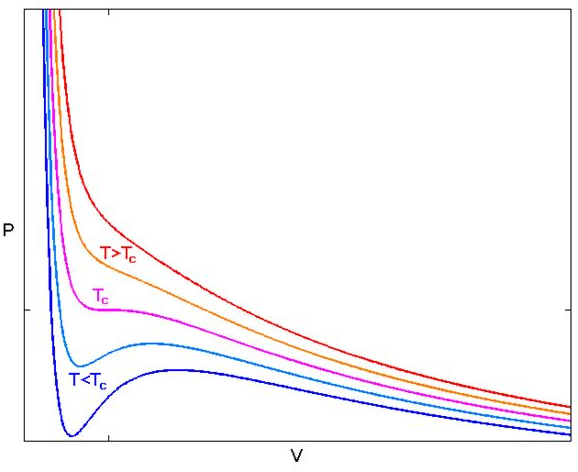
\includegraphics[scale=0.3]{IsoReal.png}
    \end{center}
\end{wrapfigure}

Isotherms have changed shapes:

Above $T_c$, real gases behave as ideal gases would

At $T_c$, have point of inflection ($p_c, T_c, V_c$)
\begin{equation*}
    \Big(\frac{\p p}{\p V}\Big)_{T_c} = 0 = \Big(\frac{\p^2 p}{\p V^2}\Big)_{T_c}
\end{equation*}
Compressibility is
\begin{equation*}
    \kappa_T = -\frac{1}{V}\Big(\frac{\p V}{\p p}\Big)_T,~ \kappa_{T_c} \to \infty
\end{equation*}
Below $T_c$, $\kappa_T$ becomes negative because $\Delta p > 0$, we have $\Delta V > 0$, pressure fluctuations can increase volume - this is unstable

\chapter{}
\section{Statistical Mechanics}
Full course at level 3, but subject is closely related to thermodynamics. Look at average atomic arrangements as opposed to behaviour of the bulk. \\
We know it is impossible to look at all atoms individually so we consider the most probable behaviour.

At thermal equilibrium, a material occupies the macrostate - has the highest number of microstates associated with it.
\begin{itemize}
    \item Macrostate - Description of material's average behaviour, i.e. what we observe
    \item Microstate - Most detailed description we have, i.e. individual arrangements
\end{itemize}

\subsection{100 coins in a box}
Open the lid after shaking, the coins are in one of $2^{100} \to 10^{30}$ arrangements. \\
Each arrangement is equally likely, if each state can have a label $[1,2,\cdots,100]$, could identify the microstate.

However, macrostate of number of heads and tails is simpler: $\approx 50H + 50T$

Each macrostate has many microstates, but there is a greater chance of seeing some arrangements.
\begin{table}[H]
    \centering
    \begin{tabular}{|c|c|c|}
        \hline
        Macro & \multicolumn{2}{c|}{Number of Microstates} \\
        \hline
        $50H + 50T$ & $\frac{100!}{(50!\times50!)}$ & $\approx 4\times10^{27}$ \\
        $53H + 47T$ & $\frac{100!}{(53!\times47!)}$ & $\approx 3\times10^{27}$ \\
        $90H + 10T$ & $\frac{100!}{(90!\times10!)}$ & $\approx 10^{13}$ \\
        $100H + 0T$ & $\frac{100!}{(100!\times0!)}$ & $1$ \\
        \hline
    \end{tabular}
\end{table}
To count distinguishable particles - number of microstates in the macrostate:
\begin{equation*}
    \Omega = \frac{N!}{\prod_{j} n_j!},~ \prod_{j}n_j! = n_1!\times n_2!\times n_3!\times\cdots\times n_n!
\end{equation*}
Total particles is $N = \sum n_j$, $n_j$ particles in a state with energy $\epsilon_j$

$N!$ total arrangements:
\begin{itemize}
    \item First particle in $N$ places
    \item Second particle in $N - 1$ places
    \item etc
\end{itemize}
Don't care how particles are arranged in state j so divide $\prod n_j!$ \\
Statistical temperature:
\begin{equation*}
    \beta = \frac{1}{k_B T} = \frac{d(\ln\Omega)}{dE}
\end{equation*}
At thermal equilibrium, the state which is most probable (highest number of microstates)
\begin{equation*}
    \text{Entropy, }S = k_B \ln\omega
\end{equation*}

\subsection{Joule Expansion of a gas}
Example of Free expansion, removing partition: $V \to 2V$ \\
One mole of gas with a constant temperature, $dU = 0$:
\begin{align*}
    dU &= \delta Q + \delta W \\
    &= T\,dS - p\,dV \\
    T\,dS &= p\,dV \\
    \Delta S &= \int_{V_0}^{2V_0} \frac{p\,dV}{T},~ pV = RT \\
    \Delta S &= \int_{V_0}^{2V_0} \frac{R}{V}\,dV = R\ln2
\end{align*}
Each molecule can now be arranged in twice the number of ways. For one mole, we have $2^{N_A}$ ways of placing the molecules so the number of microstates is $2^{N_A}$ larger:
\begin{align*}
    \Omega_{after} &= 2^{N_A}\Omega_{before} \\
    S_{after} &= k_B \ln\Omega_{after} = k_B \ln(2^{N_A}\Omega_{before}) \\
    &= k_B N_A \ln2 + k_B\ln\Omega_{before} \\
    &= k_B N_A \ln2 + S_{before} \\
    \Delta S &= k_B N_A \ln2 = R\ln2
\end{align*}
For even small systems, there are lots of microstates and factorials of large numbers. $\Omega$ has factorials of $N_A!$ \\
Striling Approximation:
\begin{equation*}
    \ln(X)! \approx X\ln(X) - X
\end{equation*}

\section{Boltzmann Distribution}
Boltzmann is a probability distribution telling us the probability of finding particle with $\epsilon_j$ at temperature T
\begin{equation*}
    P(\epsilon_j) \propto \exp\Big(\frac{-\epsilon_j}{k_B T}\Big) = \frac{\exp\big(\tfrac{-\epsilon_j}{k_B T}\big)}{\sum_{j} \exp\big(\tfrac{-\epsilon_j}{k_B T}\big)}
\end{equation*}
The sum on the bottom is the partition function:
\begin{equation*}
    Z = \sum_{j} \exp\Big(\frac{-\epsilon_j}{k_B T}\Big)
\end{equation*}
This ensure normalisation such that
\begin{equation*}
    \sum_{j} P(\epsilon_j) = 1
\end{equation*}
At thermal equilibrium, there are three conditions:
\begin{enumerate}
    \item Fixed particle number
            \begin{equation*}
                N = \sum_j n_j ~;~ dN = \sum dn_j = 0
            \end{equation*}
    \item Fixed total energy
            \begin{equation*}
                E = \sum_{j} \epsilon_j n_j ~;~ dE = \sum \epsilon_j dn_j = 0
            \end{equation*}
    \item The most probable macrostate has the most microstates so $d\Omega = 0$. This is equivalent to
            \begin{equation*}
                \sum_{j} (\ln n_j)\,dn_j = 0
            \end{equation*}
\end{enumerate}
For all conditions, Lagrange multipliers solve having a number of conditions zero simultaneously
\begin{align*}
    \sum_{j}& (\alpha\,dn_j + \beta\epsilon_j\,dn_j + (\ln n_j)\,dn_j) = 0 \\
    \sum_{j}& dn_j (\alpha + \beta\epsilon_j + \ln n_j) = 0
\end{align*}
To hold for all j:
\begin{align*}
    (\alpha &+ \beta\epsilon_j + \ln n_j) = 0 \\
    n_j &= \exp(-\alpha - \beta\epsilon_j) = A\exp\Big(\frac{-\epsilon_j}{k_B T}\Big) \\
    \beta &= \frac{1}{k_B T} ~;~ A = \frac{1}{Z} = \frac{1}{\sum_{j} \exp\big(\tfrac{-\epsilon_j}{k_B T}\big)}
\end{align*}

\section{Partition Function}
$Z$ links the subjects. It is a zipped up version of all thermodynamic properties \\
It can be shown that
\begin{align*}
    S &= k_B T\ln Z + \frac{U}{T} \\
    U &= -\frac{d(\ln Z)}{d\beta} = k_B T^2 \frac{d(\ln Z)}{dT} ~;~ U \propto E = \sum_{j} n_j \epsilon_j
\end{align*}
This tells us that
\begin{align*}
    F &= -k_B T\ln Z \\
    Z &= \exp(-\beta F)
\end{align*}

\section{Quantum Particles}

\subsection{Wavefunctions}
From Quantum mechanics, we have two types of indistinguishable particle, bosons and fermions.
Look at their wavefunctions where swapping particles either leaves the wavefunction unchanged, or introduces an overall minus sign.
In both cases, the probability of state occupation doesn't change. Considering the two particle wavefunction $\psi(1,2)$ where 1, 2 represent the coordinates of each particle.
If the particles are indistinguishable, changing the patticle labels will not result in a change to the physical oberservables.
The solution of the Schrodinger for the two particles can be written as the product of the one-particle wavefunctions, $\psi(1,2) = \psi_{a}(1)\psi_{b}(2)$, where $a$ and $b$ are the values of state label.

Symmetry in Bosons, any number in a quantum state:
\begin{equation*}
    \psi_S (1,2) = \frac{1}{\sqrt{2}}[\psi_a(1)\psi_b(2) + \psi_a(2)\psi_b(1)]
\end{equation*}
Anti-symmetry in Fermions, from the Pauli exclusion principle, can only have one particle per quantum state (two per energy level as we have spin up and spin down)
\begin{equation*}
    \psi_A(1,2) = \frac{1}{\sqrt{2}}[\psi_a(1)\psi_b(2) - \psi_a(2)\psi_b(1)]
\end{equation*}
You can show that $\psi_S(1,2) = \psi_S(2,1)$ and $\psi_A(1,2) = -\psi_A(2,1)$

\subsection{Arrangements of Indistinguishable Particles}
If particles are indistinguishable, e.g. gases, it is better to consider distribution functions.
Here we look at energy levels, as opposed to state.
In other words, lots of energy levels are collected together into bundles with the $i^{th}$ bundle have $g_i$ states, or energy levels, containing $n_i$ particles associated with it.

The Maxwell Boltzmann distribution for a classical gas:
\begin{equation*}
    f_{MB}(\epsilon) = A\exp\Big(\frac{-\epsilon}{k_B T}\Big)
\end{equation*}
We have many more energy levels, so $\epsilon$ is now continious \\
$f(\epsilon)$ - distribution function, probability a state having energy $\epsilon$ is occupied \\
$g(\epsilon)d\epsilon$ - density of states, how many energy levels are in the range, $d\epsilon$ \\
$n(\epsilon)d\epsilon = f(\epsilon)g(\epsilon)d\epsilon$ - number of particles in the energy interval $d\epsilon$

\begin{wrapfigure}{r}{0.4\textwidth}
    \begin{center}
        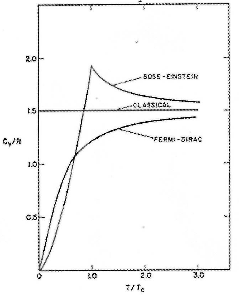
\includegraphics[scale=0.6]{BoseEinstein.png} \\
        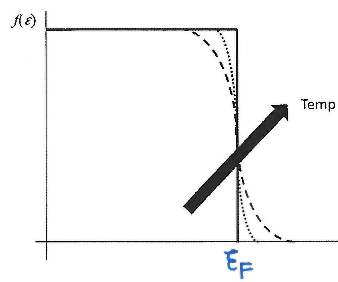
\includegraphics[scale=0.5]{FermiDirac.png} \\
        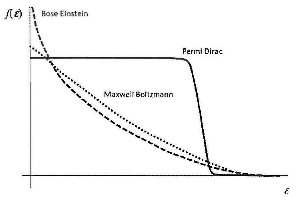
\includegraphics[scale=0.6]{Limits.png}
    \end{center}
\end{wrapfigure}

\textbf{Bose-Einstein Distribution}
\begin{equation*}
    f_{BE}(\epsilon) = \frac{1}{\exp\big(\tfrac{\epsilon - \mu}{k_B T}\big) - 1}
\end{equation*}
$\mu$ is the chemical potential, i.e. the energy to add one particle \\
As $T \to 0$, $\mu \to \epsilon_0$ of the lowest state:
\begin{align*}
    \lim_{T\to0}& \exp\Big(\frac{\epsilon - \mu}{k_B T}\Big) = 1 \\
    f_{MB} &\to \frac{1}{0} \to \infty
\end{align*}
All particles migrate to the lowest energy state. \\
2nd order phase change for heat capacity.

\textbf{Fermi-Dirac Distribution}
\begin{equation*}
    f_{FD}(\epsilon) = \frac{1}{\exp\big(\tfrac{\epsilon - \epsilon_F}{k_B T}\big) + 1}
\end{equation*}
$\epsilon_F$ is the Fermi energy \\
At $T = 0$K all states are occupied to the Fermi energy \\
Raise T moves particlea above $\epsilon_F$ \\
At $T = 0$K:
\begin{equation*}
    f_{FD}(\epsilon) =
    \begin{cases}
        \epsilon \leq \epsilon_F & = 1 \\
        \epsilon > \epsilon_F & = 0
    \end{cases}
\end{equation*}

\textbf{Classical Limits}

Low probability of state occupation - many more states than particles, so quantum effects are irrelevant

Fermi-Dirac $\propto$ Bose-Einstein tend towards Maxwell-Boltzmann
\end{document}
